\documentclass[12pt,a4paper,oneside]{report}

% --- 1. Lingua, codifica e font -----------------------------------------------
\usepackage[T1]{fontenc}
\usepackage[utf8]{inputenc}
\usepackage[english,french,italian]{babel}
\usepackage{lmodern}
\usepackage[autostyle,italian=guillemets]{csquotes} % Per \enquote{...} (Cap. 4)

% --- 2. Geometria pagina e interlinea -----------------------------------------
\usepackage[a4paper,top=3cm,bottom=3cm,inner=3.5cm,outer=2.5cm]{geometry}
\usepackage{setspace}
\onehalfspacing

% --- 3. Matematica, numeri e unità di misura ----------------------------------
\usepackage{amsmath}
\usepackage{amssymb}
\usepackage{siunitx} % Per \num{...} e \SI{...}{\percent} (Cap. 4)
\sisetup{output-decimal-marker={,}, group-separator={.}, group-minimum-digits=5}

% --- 4. Grafica, TikZ, tabelle e posizionamento -------------------------------
\usepackage{graphicx}
\usepackage{float}      % Per [H] (Cap. 3)
\usepackage{booktabs}   % Per \toprule, \midrule, \bottomrule
\usepackage{tabularx}   % Per tabelle tabularx (Cap. 4)
\usepackage{multirow}   % Per \multirow (Cap. 4)
\usepackage{caption}    % Per didascalie (Cap. 4)
\usepackage{subcaption} % Per \begin{subfigure} (Cap. 4)
\usepackage{xcolor}
\usepackage{tikz}       % Per i diagrammi CRISP-DM (Cap. 1)
\usepackage[section]{placeins}

\usetikzlibrary{arrows.meta}
\usetikzlibrary{positioning}
\usetikzlibrary{shapes.symbols, calc}

% --- 5. Bibliografia ----------------------------------------------------------
\usepackage[backend=biber]{biblatex}

% --- 6. Comandi personalizzati del Capitolo 4 ---------------------------------
\DeclareRobustCommand{\file}[1]{\texttt{\detokenize{#1}}}
\DeclareRobustCommand{\campo}[1]{\texttt{\detokenize{#1}}}

% --- 7. Collegamenti e riferimenti incrociati (SEMPRE per ultimi!) ------------
\usepackage[hidelinks]{hyperref} % Necessario per \texorpdfstring nei titoli del Cap. 4
\usepackage[italian,capitalise,noabbrev]{cleveref}
\crefname{chapter}{Capitolo}{Capitoli}
\crefname{section}{Sezione}{Sezioni}
\crefname{table}{Tabella}{Tabelle}
\crefname{figure}{Figura}{Figure}
\crefname{appendix}{Appendice}{Appendici}

% --- Metadati del documento ---------------------------------------------------
\title{Tesi di Laurea}
\author{Misael Monaco}
\date{Settembre 2026}

\begin{document}

\maketitle

\tableofcontents

\clearpage

% =============================================================================
% CAPITOLO 1
% =============================================================================
% =============================================================================
% CAPITOLO 1
% =============================================================================

\chapter{Introduzione}

\section{Contesto e motivazione}
\label{sec:contesto}

Il Regolamento (UE) 2024/1689 \cite{aiact2024}, noto anche come AI Act, rappresenta il primo quadro normativo orizzontale al mondo per la regolamentazione dell'intelligenza artificiale. La portata del testo è monumentale: esteso su oltre 144 pagine della Gazzetta Ufficiale dell'Unione Europea, il regolamento si articola in 180 considerando, 113 articoli e 13 allegati tecnici. Il legislatore comunitario ha adottato un approccio basato sul rischio (\textit{risk-based approach}), introducendo una classificazione piramidale che va dal rischio inaccettabile (pratiche vietate con decorrenza a 6 mesi dall'entrata in vigore), ai sistemi di IA per finalità generali (GPAI, con obblighi a 12 mesi), fino ai sistemi ad alto rischio, per i quali è prevista la piena efficacia tra i 24 e i 36 mesi.

Le ripercussioni operative e i rischi di non conformità sono senza precedenti per il settore tecnologico: le sanzioni pecuniarie possono raggiungere i 35 milioni di euro o fino al 7\% del fatturato globale mondiale annuo per la violazione delle pratiche vietate (Art.~5), e fino a 15 milioni di euro o al 3\% del fatturato per l'inadempimento degli obblighi relativi ai sistemi ad alto rischio e ai requisiti di trasparenza.

Gli obblighi previsti non ricadono su un unico soggetto generico, ma sono meticolosamente distribuiti su una pluralità di figure lungo l'intera catena del valore (fornitori, \textit{deployer}, importatori, distributori, rappresentanti autorizzati, organismi notificati e autorità di vigilanza) e si estendono lungo tutto il ciclo di vita del sistema, dalla progettazione al monitoraggio post-immissione sul mercato. Ciascun ruolo è gravato da vincoli operativi specifici:
\begin{itemize}
    \item \textbf{Per un fornitore di un sistema ad alto rischio} (come un algoritmo di screening automatizzato delle candidature lavorative o di credit scoring, inquadrati nell'Allegato III), la conformità non è un mero adempimento documentale, ma un vincolo architetturale: l'Art.~9 impone un sistema continuo di gestione dei rischi; l'Art.~10 obbliga a rigorose pratiche di \textit{data governance} sui dati di addestramento e validazione per mitigare distorsioni statistiche (\textit{bias}); l'Art.~12 richiede la registrazione automatica e continua dei log operativi per garantire tracciabilità; l'Art.~14 prescrive la predisposizione tecnica di meccanismi di sorveglianza umana (\textit{human oversight}), quali interfacce di arresto e override.
    \item \textbf{Per un deployer}, l'Art.~26 stabilisce l'obbligo di impiegare il sistema nel rispetto delle istruzioni d'uso, assicurare la pertinenza dei dati di input e conservare i log generati automaticamente per un periodo minimo di almeno sei mesi.
\end{itemize}

Attualmente, la traduzione di questo articolato testo normativo in requisiti operativi concreti — ovvero la definizione puntuale di \textit{chi} debba fare \textit{cosa}, in quale momento del ciclo di vita e tenendo conto di quali rinvii interni — rappresenta una sfida critica per organizzazioni ed esperti del settore. Il regolamento crea infatti una fitta rete di interdipendenze: l'Art.~16 (che enumera gli obblighi dei fornitori) rinvia a cascata ad oltre dieci articoli distinti (Artt.~9--15, 43, 49, 72) e ai dettagli tecnici dell'Allegato IV. Oggi questo processo si basa quasi interamente su audit manuali condotti da giuristi ed esperti di conformità, risultando in un'attività dispendiosa in termini di tempo, onerosa (con costi stimati nell'ordine di decine o centinaia di migliaia di euro per singolo sistema) e strutturalmente soggetta a incongruenze, omissioni e disallineamenti tra l'interpretazione giuridica e l'effettiva implementazione software.

Tuttavia, analizzando la stesura del regolamento, emerge come il testo presenti una struttura linguistica e logica piuttosto riconoscibile: le disposizioni normative seguono pattern ricorrenti composti da un soggetto obbligato esplicito, un verbo deontico (\textit{deve}, \textit{garantisce}, \textit{è tenuto a}), l'oggetto dell'azione e i relativi rinvii ad altri articoli. Scomposto a grana fine nel presente lavoro, il testo consolidato produce \textbf{1.775 proposizioni normative atomiche} (1.852 nella versione iniziale comprensiva del paratesto), delle quali \textbf{1.172 aventi rilevanza normativa diretta} (1.027 negli articoli 1--112 e 145 negli allegati tecnici). Questa intrinseca regolarità strutturale rende il testo giuridico particolarmente adatto all'applicazione congiunta di tecniche di \textit{Natural Language Processing} (NLP) e di estrazione automatica della conoscenza.

Da queste premesse nasce l'idea fondante della presente tesi: progettare e sviluppare una \textit{pipeline} automatizzata capace di analizzare il testo normativo e tradurlo bottom-up in un catalogo di componenti software tracciabili, colmando il divario tra prescrizione normativa e architettura software di conformità.


\section{Obiettivi della tesi}
\label{sec:obiettivi}
Il lavoro persegue tre macro-obiettivi:

\begin{enumerate}
\item \textbf{Costruire una pipeline riproducibile} che trasformi il testo del regolamento, così come pubblicato su EUR-Lex, in un dataset strutturato di proposizioni normative, ciascuna classificata per tipo di obbligo, livello di rischio e soggetto obbligato, arricchita con entità di dominio (attori, autorità, riferimenti normativi) estratte automaticamente.

\item \textbf{Validare l'accuratezza dei classificatori automatici}: la valutazione riguarda sia il \textbf{classificatore deterministico delle proposizioni} (per modalità deontica e livello di rischio), scelto per aderire in modo ispezionabile alle formule legistiche codificate dell'UE in assenza di dataset pre-annotati sull'AI Act, sia i \textbf{modelli di riconoscimento delle entità (NER)}. Per questi ultimi sono stati selezionati e posti a confronto tre paradigmi: una baseline statistica generalista (\emph{spaCy}), scelta come controllo negativo fuori dominio; un sistema simbolico a regole (\emph{gazetteer} ed espressioni regolari), scelto per sfruttare il vocabolario chiuso dei ruoli definiti dall'Articolo~3; e modelli neurali Transformer pre-addestrati su corpora giuridici (\emph{Italian-Legal-BERT}, \emph{LEGAL-BERT} e \emph{JuriBERT}), scelti per verificare se la rappresentazione contestuale del linguaggio legale consenta di superare i limiti sintattici delle regole in un regime di scarsità di dati annotati (\emph{weak} e \emph{strong supervision}). Tutti i moduli vengono valutati su campioni annotati manualmente: ogni stima è calcolata su proposizioni mai usate per mettere a punto il sistema, annotate alla cieca senza vederne le predizioni (\emph{blind annotation}).

\item \textbf{Verificare cosa rivelano della struttura di un atto normativo tecniche diverse} (Topic Modeling, Topological Data Analysis, Formal Concept Analysis) e se questa struttura permetta di ricavare, dal basso ed in modo riproducibile, una ipotesi di architettura software per la conformità.
\end{enumerate}


\section{Domande di ricerca}
\label{sec:domande}
\begin{itemize}
    \item \textbf{$\mathcal{D}_1$ --- Regole o modello neurale?}
    Il riconoscimento delle entità è stato realizzato in due modi: con regole simboliche basate su espressioni regolari e gazetteer, e con Italian-Legal-BERT, un modello linguistico specializzato sul diritto italiano addestrato con supervisione debole. La domanda è se il deep learning superi le regole o se ne erediti i limiti sistematici.
    \item \textbf{$\mathcal{D}_2$--- Quali regole possono essere recuperate dal testo e costruite in un modello concettuale?} Nel dettato normativo, diverse prescrizioni tecniche risultano prive di un attore sintattico esplicito all'interno della singola frase, poiché demandano l'individuazione del soggetto responsabile alla struttura gerarchica dell'atto. La domanda è quali regole formali di inferenza e di eredità contestuale possano essere estratte dal testo e integrate nel modello concettuale (\emph{Formal Concept Analysis}) per recuperare tali legami impliciti --- consentendo di ricondurre nel catalogo anche disposizioni centrali altrimenti escluse, come la governance dei dati (Art.~10) --- e come validarne la tenuta rispetto a generalizzazioni spurie.
    \item \textbf{$\mathcal{D}_3$ --- Quale architettura software impone la regolamentazione (se ne esiste una)?} Non è scontato a priori che un testo legislativo contenga una struttura modulare traducibile in componenti software, né che i raggruppamenti estratti riflettano una proprietà intrinseca della norma anziché un artefatto algoritmico. La domanda è se dall'aggregazione di cluster bivariati $\text{attore} \times \text{tema}$ emerga un'architettura di conformità ben definita, come si formalizzino tali gruppi e quanto i componenti risultanti siano stabili al variare dei parametri ($k$, soglia di supporto), del modello di estrazione e della lingua (italiano, inglese e francese).
\end{itemize}

\section{Contributo scientifico e applicativo}
\label{sec:contributo}
Le tecniche impiegate nella tesi si fondano su letterature consolidate. Il lavoro ne propone un impiego congiunto sul medesimo testo normativo, articolando il contributo su due piani:

\begin{itemize}
    \item \textbf{Pipeline e dataset}. La realizzazione di una pipeline \emph{end-to-end} riproducibile che trasforma il testo grezzo dell'AI Act in un dataset strutturato di proposizioni normative (1.175 totali, di cui 1.172 prescrittive in italiano, replicato sulle versioni inglese e francese), arricchito con coordinate strutturali, tipo di obbligo, livello di rischio, entità astratte(attori, autorità, rinvii), profilo tematico NMF, contesto formale binario e campioni \emph{gold} annotati manualmente alla cieca.
    
    \item \textbf{Metodologia}. Il risultato principale riguarda il confronto tra regex e modello neurale. Il modello, addestrato sulle etichette prodotte dalle regex (\textit{silver labels}), ne eredita gli errori sistematici: il suo vantaggio iniziale dipendeva da bug delle regole e, una volta corretti, i due sistemi convergono alla parità statistica ($0{,}924$ contro $0{,}919$ sul round cieco, $p = 1{,}00$, e $0{,}954$ contro $0{,}953$ pooled). Un modello addestrato solo su supervisione debole non può superare il proprio supervisore simbolico.
    La tesi documenta inoltre i rischi metodologici della valutazione: il classificatore del tipo di obbligo raggiunge il $67{,}6\%$ di accuratezza ($89{,}2\%$ sul rischio) su un campione di test indipendente; per il NER, la separazione netta tra annotatore e predizioni ha eliminato i bias di ancoraggio.
    
    \item \textbf{Applicativo}. Un catalogo di 9 componenti software derivato dal testo dell'AI Act, organizzato per stadio del ciclo di vita di un sistema di IA e tracciabile fino agli articoli. I componenti restano stabili al variare dei parametri, anche se il numero di cluster intermedi varia ($\mathcal{D}_3$). Il punto cieco principale del catalogo, la data governance, è stato risolto comprendendo il regime impersonale della Sezione 2 del Capo III: l'Art.~16 assegna infatti la responsabilità al fornitore. Una regola di eredità recupera 54 proposizioni della sezione (di cui 27 dell'Art.~10), con una precisione del $96{,}3\%$ (52 su 54 corrette) verificata manualmente a cieco.
\end{itemize}



\section{Perimetro del lavoro ed esclusioni}
La tesi analizza un solo atto, il Regolamento (UE) 2024/1689, nel testo consolidato pubblicato nella Gazzetta Ufficiale del 12 luglio 2024, scaricato da EUR-Lex e mantenuto congelato. Aggiornamenti successivi del testo non sono considerati. La lingua principale è l'italiano; inglese e francese sono utilizzati per il controllo incrociato comparativo.\\[0.5cm]
\textbf{Cosa rientra nell'analisi}
\begin{itemize}
    \item Il testo degli articoli (1--112) e dei tredici allegati tecnici (I--XIII). I considerando, le 58 note a piè di pagina e la formula finale con le firme sono esclusi: i considerando spiegano le ragioni della norma ma non dispongono obblighi vincolanti, le note sono solo riferimenti bibliografici.
    \item L'unità minima di analisi è la singola proposizione normativa atomica.
    \item Tre categorie di entità: gli attori a cui la norma assegna obblighi, le autorità pubbliche e i rinvii normativi.
\end{itemize}
\textbf{Che cosa non rientra}
\begin{itemize}
    \item \textbf{L'interpretazione giuridica vincolante}. La tesi estrae e organizza ciò che il testo prescrive letteralmente; non stabilisce dottrina né pareri legali.
    \item \textbf{Le fonti secondarie}. Atti delegati, atti di esecuzione, linee guida dell'AI Office e norme tecniche armonizzate (CEN/CENELEC) non sono inclusi nel corpus.
    \item \textbf{Uno strumento software finito pronto all'uso}. Il catalogo è la proposta formale di un'architettura ricavata dal testo, non un sistema software già implementato.
    \item \textbf{I modelli generativi per l'estrazione primaria}. Il confronto empirico è focalizzato tra regole formali e modelli discriminativi di dominio (Legal-BERT); i Large Language Models sono trattati nello stato dell'arte e nelle prospettive future.
\end{itemize}

\newpage

\begin{figure} [!t]
    \centering
    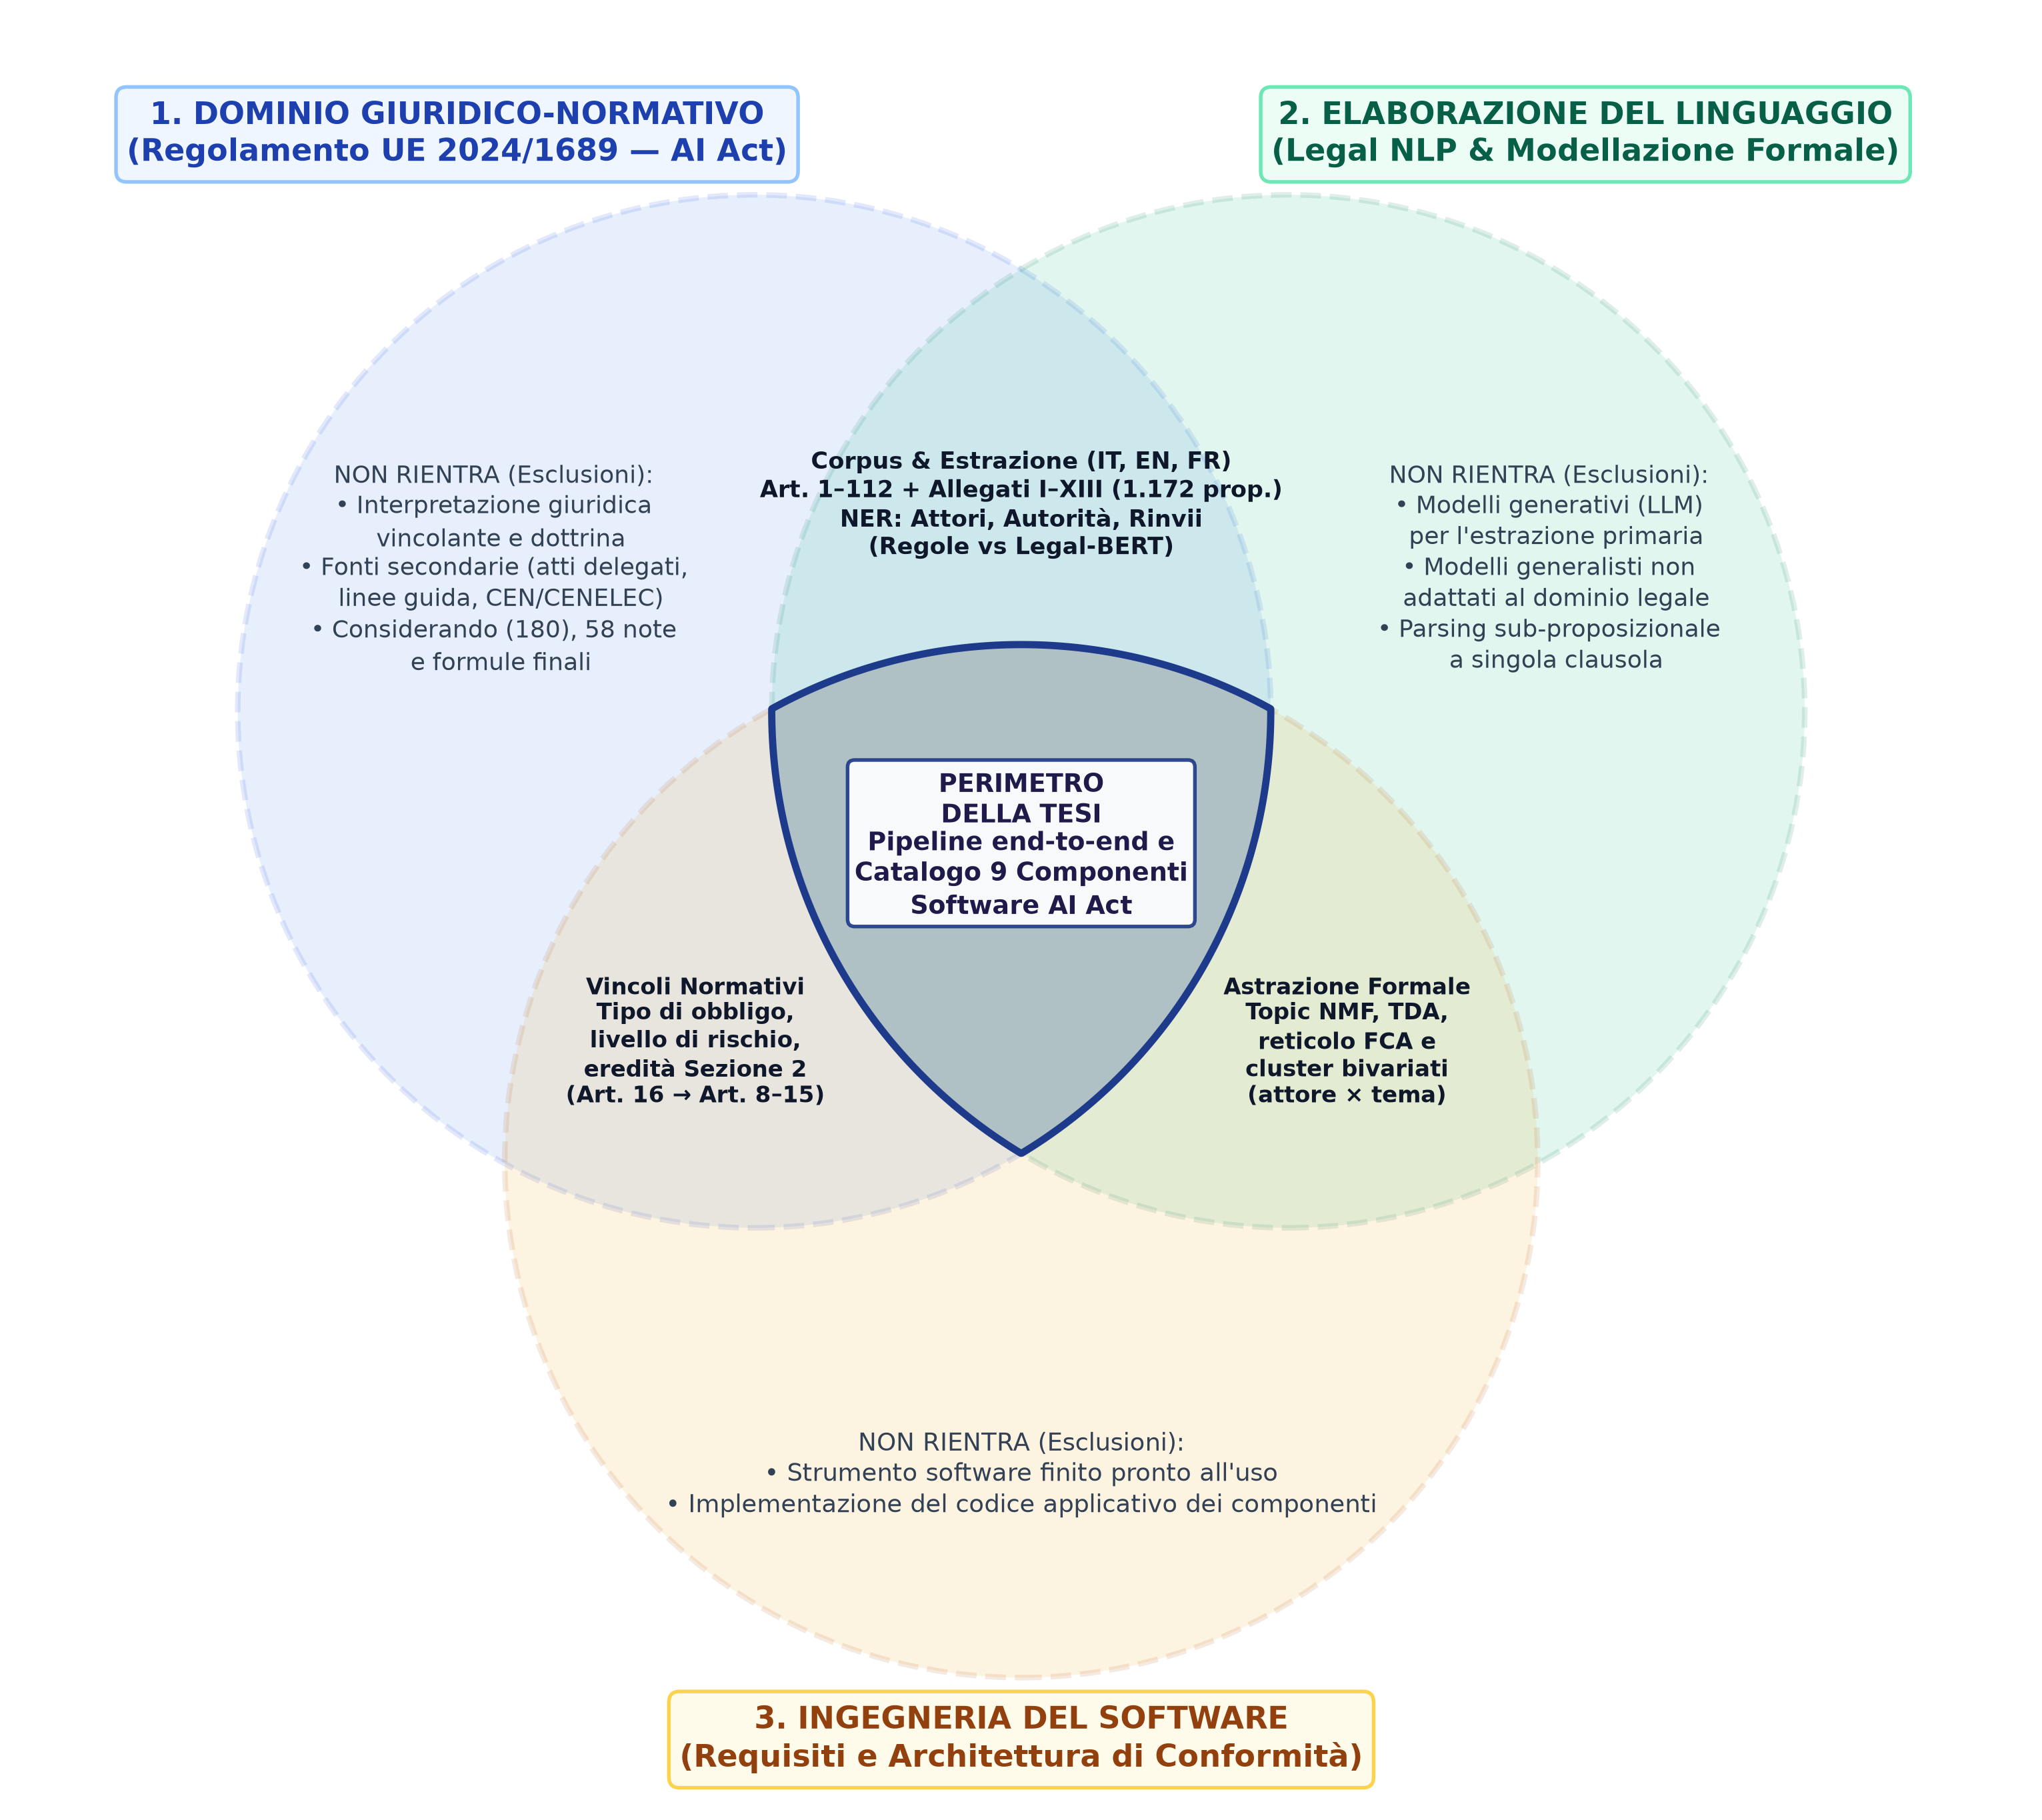
\includegraphics[width=0.8\linewidth]{venn_perimetro.png}
    \caption[Diagramma di Venn del perimetro della tesi]{Rappresentazione insiemistica del perimetro del lavoro: le regioni esterne tratteggiate individuano le esclusioni esplicite, le intersezioni intermedie gli elementi analitici inclusi e il nucleo centrale il contributo complessivo della tesi.}
    \label{fig:venn_perimetro}
\end{figure}

La Figura \ref{fig:venn_perimetro} riassume visivamente il confine all'intersezione tra dominio normativo, \emph{Legal NLP} e ingegneria del software. Le regioni esterne tratteggiate isolano gli elementi esclusi (fonti secondarie, paratesto e interpretazione dottrinale; modelli generativi; sviluppo di codice applicativo), mentre le intersezioni intermedie raccordano il testo prescrittivo, i modelli di estrazione e l'astrazione formale che definisce il perimetro della tesi: la pipeline \emph{end-to-end}, il catalogo dei 9 componenti architetturali.
 

\section{Quadro metodologico: la pipeline come processo CRISP-DM}
\subsection{Perché CRISP-DM}
CRISP-DM (\textit{Cross-Industry Standard Process for Data Mining}; Chapman et al., 2000; Wirth e Hipp, 2000) descrive un progetto di analisi dei dati in sei fasi: comprensione del problema, comprensione dei dati, preparazione dei dati, modellazione, valutazione e messa in uso. Le fasi non sono strettamente sequenziali: il modello prevede ritorni espliciti alle fasi precedenti quando la valutazione mostra un problema.

È una cornice adatta a questo lavoro non per analogia, ma perché quei ritorni sono avvenuti davvero, cinque volte ((Tabella~\ref{tab:dettaglio_iterazioni}). In ognuno, un'anomalia emersa valutando i risultati ha richiesto di correggere una fase a monte, e la correzione è stata poi verificata su dati non utilizzati per ricavarla.

\subsection{Le sei fasi applicate alla pipeline}

\begin{figure}[htbp]
\centering
\resizebox{\textwidth}{!}{%
\begin{tikzpicture}[
    scale=0.95,
    font=\small\sffamily,
    transarrow/.style={-{Stealth[length=3mm]}, line width=2pt, draw=black},
    calloutline/.style={line width=0.8pt, draw=black!80},
    chevron/.style={line width=1pt, draw=black!85},
    callout/.style={
        text width=3.9cm, 
        font=\scriptsize, 
        align=center, 
        inner sep=1pt
    }
]

\definecolor{cBusiness}{RGB}{68, 114, 196}
\definecolor{cDataUnd}{RGB}{237, 125, 49}
\definecolor{cDataPrep}{RGB}{128, 130, 133}
\definecolor{cModeling}{RGB}{255, 230, 0}
\definecolor{cEvaluation}{RGB}{0, 176, 240}
\definecolor{cDeployment}{RGB}{0, 176, 80}

% RIGA 1: FASI 1, 2, 3
\filldraw[chevron, fill=cBusiness] 
    (0,0) arc (-90:90:0.6cm and 1.1cm) -- (4.2,2.2) -- (4.2,0) -- cycle;
\node[align=center, text=black, font=\large\bfseries] at (2.4, 1.1) {Business\\Understanding};

\filldraw[chevron, fill=cDataUnd] 
    (5.4,0) arc (-90:90:0.6cm and 1.1cm) -- (9.6,2.2) -- (9.6,0) -- cycle;
\node[align=center, text=black, font=\large\bfseries] at (7.8, 1.1) {Data\\Understanding};

\filldraw[chevron, fill=cDataPrep] 
    (10.8,0) arc (-90:90:0.6cm and 1.1cm) -- (15.0,2.2) -- (15.0,0) -- cycle;
\node[align=center, text=black, font=\large\bfseries] at (13.2, 1.1) {Data\\Preparation};

\draw[transarrow] (4.2, 1.1) -- (5.4, 1.1);
\draw[transarrow] (9.6, 1.1) -- (10.8, 1.1);

% RIGA 2: FASI 4, 5, 6
\draw[transarrow] (15.0, 1.1) -- (15.8, 1.1) -- (15.8, -1.9) -- (15.0, -1.9);

\filldraw[chevron, fill=cModeling] 
    (10.8,-3.0) arc (-90:90:0.6cm and 1.1cm) -- (15.0,-0.8) -- (15.0,-3.0) -- cycle;
\node[align=center, text=black, font=\large\bfseries] at (13.2, -1.9) {Modeling};

\filldraw[chevron, fill=cEvaluation] 
    (5.4,-3.0) arc (-90:90:0.6cm and 1.1cm) -- (9.6,-0.8) -- (9.6,-3.0) -- cycle;
\node[align=center, text=black, font=\large\bfseries] at (7.8, -1.9) {Evaluation};

\filldraw[chevron, fill=cDeployment] 
    (0,-3.0) arc (-90:90:0.6cm and 1.1cm) -- (4.2,-0.8) -- (4.2,-3.0) -- cycle;
\node[align=center, text=black, font=\large\bfseries] at (2.4, -1.9) {Deployment};

\draw[transarrow] (10.8, -1.9) -- (9.6, -1.9);
\draw[transarrow] (5.4, -1.9) -- (4.2, -1.9);

% CALLOUT SUPERIORI
\draw[calloutline] (1.2, 2.2) -- (1.2, 3.1) -- (1.8, 3.1);
\node[callout, anchor=south] at (2.1, 3.15) {
    \textbf{Analisi requisiti:}\\
    Mappatura conformità AI Act in requisiti software operativi
};

\draw[calloutline] (6.6, 2.2) -- (6.6, 3.1) -- (7.2, 3.1);
\node[callout, anchor=south] at (7.5, 3.15) {
    \textbf{Analisi corpus EUR-Lex:}\\
    Studio complessità su 113 articoli, 180 considerando e 13 allegati
};

\draw[calloutline] (12.0, 2.2) -- (12.0, 3.1) -- (12.6, 3.1);
\node[callout, anchor=south] at (12.9, 3.15) {
    \textbf{Segmentazione e NER:}\\
    1.775 proposizioni atomiche, classi deontiche e gazetteer entità
};

% CALLOUT INFERIORI
\draw[calloutline] (13.6, -3.0) -- (13.6, -3.9) -- (13.0, -3.9);
\node[callout, anchor=north] at (12.9, -3.95) {
    \textbf{NLP e Rappresentazione:}\\
    Topic Modeling (NMF), omologia persistente (TDA) e reticolo (FCA)
};

\draw[calloutline] (8.2, -3.0) -- (8.2, -3.9) -- (7.6, -3.9);
\node[callout, anchor=north] at (7.5, -3.95) {
    \textbf{Validazione in due round:}\\
    Campioni ciechi indipendenti, stima onesta e fix anti-circolarità
};

\draw[calloutline] (2.8, -3.0) -- (2.8, -3.9) -- (2.2, -3.9);
\node[callout, anchor=north] at (2.1, -3.95) {
    \textbf{Sintesi architetturale:}\\
    Catalogo di 9 componenti tracciabili e diagrammi interattivi
};

\end{tikzpicture}
}
\caption{La pipeline metodologica inquadrata nelle sei fasi del framework CRISP-DM.}
\label{fig:pipeline_crisp_dm}
\end{figure}

\subparagraph{Comprensione del problema (Business Understanding)}
L'obiettivo è quello di rendere interrogabile un testo normativo lungo e stratificato, a supporto di una analisi di conformità ad oggi in parte manuale. Due criteri hanno guidato il lavoro:
\begin{itemize}
    \item le prestazioni dei componenti automatici devono essere stimate su dati mai usati per metterli a punto;
    \item il catalogo finale deve restare tracciabile fino alle singole proposizioni e agli articoli da cui deriva.
\end{itemize}

\subparagraph{Comprensione dei dati (Data Understanding)}
Il testo del Regolamento è stato scaricato da EUR-Lex e suddiviso nei singoli commi e punti elenco: 1.353 record (1.456 nella segmentazione iniziale). Una prima classificazione automatica mostra una peculiarità linguistica: l'italiano giuridico esprime l'obbligo soprattutto al presente indicativo (\textit{«il fornitore compila...»}) anziché con formule deontiche canoniche (\textit{«deve»}). La classe «obbligo positivo» è pertanto soggetta a forte dispersione sintattica.

\subparagraph{Preparazione dei dati (Data Preparation)}
\begin{itemize}
    \item \textbf{Segmentazione} dei paragrafi in proposizioni normative: 1.775 complessive, di cui 1.172 aventi valore normativo primario.
    \item \textbf{Classificazione} di ciascuna proposizione per tipo di obbligo e livello di rischio esplicito.
    \item \textbf{Riconoscimento delle entità}: attori, autorità e rinvii normativi, con regole formali e con il modello neurale Italian-Legal-BERT.
    \item \textbf{Costruzione del contesto formale}: una matrice binaria di 1.171 proposizioni $\times$ 70 attributi che associa ad ogni proposizione le sue proprietà, passaggio chiave verso la modellazione formale.
\end{itemize}

\subparagraph{Modellazione (Modeling)}
\begin{itemize}
    \item \textbf{Topic modeling} con NMF: estrazione di 10 temi latenti ($k=10$).
    \item Sull'output di NMF operano tre tecniche:
    \begin{itemize}
        \item \textbf{analisi topologica} (TDA) dello spazio tematico mediante omologia persistente;
        \item \textbf{analisi dei concetti formali} (FCA) per strutturare la gerarchia concettuale;
        \item \textbf{clustering bivariato attore $\times$ tema}, base analitica del catalogo software.
    \end{itemize}
\end{itemize}

\subparagraph{Valutazione (Evaluation)}
La fase metodologicamente cardine. Ogni componente è valutato su campioni indipendenti annotati a mano, documentando il superamento delle distorsioni iniziali.

\begin{table}[htbp]
    \centering
    \caption{Valutazione dei componenti automatici e superamento delle stime distorte}
    \label{tab:valutazione_modelli}
    \begin{tabular}{|p{3.2cm}|p{2.1cm}|p{4.2cm}|p{3.1cm}|}
        \hline
        \textbf{Componente} & \textbf{Prima stima} & \textbf{Problema scoperto} & \textbf{Stima finale} \\
        \hline
        Classificatore tipo di obbligo & 98\% & Circolarità: campione di test contaminato con le regole & 67,6\% (89,2\% su rischio) su campione cieco \\
        \hline
        NER a regole & F1 0,86 & Ancoraggio: annotazione condizionata dalle predizioni & 0,77 alla cieca; 0,87 su terzo set dopo 4 fix \\
        \hline
        Regole vs Legal-BERT & BERT migliore ($p = 0{,}039$) & BERT eredita e riproduce i bug delle silver label & Parità statistica su round cieco ($p = 1{,}00$) \\
        \hline
    \end{tabular}
\end{table}

\subparagraph{Messa in uso (Deployment)}
I cluster bivariati attore $\times$ tema (16 in italiano, 18 in inglese e francese) sono aggregati nel catalogo di 9 componenti software, disposti lungo le 4 fasi del ciclo di vita dell'IA. Come precisato al \ref{sec:contributo}, è la proposta formale di un'architettura software di conformità, non un sistema operativo realizzato.

\begin{figure}[htbp]
    \centering
    \small In ciascuna delle cinque iterazioni, la correzione è stata scritta nella fase di destinazione e poi verificata su dati non usati per ricavarla. L'ordine cronologico è (a), (b), (c), (e), (d). \par\vspace{0.4cm}
    
    \begin{tikzpicture}[
        box/.style={draw=black, thick, fill=black!90, text=white, align=center, 
                    minimum width=3.4cm, minimum height=0.74cm, font=\sffamily\footnotesize},
        arrow/.style={-{Latex[length=2.2mm, width=1.5mm]}, thick, draw=black},
        dashed_arrow/.style={-{Latex[length=2.2mm, width=1.5mm]}, thick, dashed, draw=black!85},
        lbl/.style={fill=black!75, text=white, font=\scriptsize\sffamily, align=center, inner sep=2.5pt, rounded corners=2pt}
    ]

    % Nodi principali
    \node[box] (step1) at (0, 0) {1. Comprensione del problema};
    \node[box] (step2) at (0, -1.15) {2. Comprensione dei dati};
    \node[box] (step3) at (0, -2.3) {3. Preparazione dei dati};
    
    % Modello a diamante
    \node[box] (step4) at (-2.3, -4.4) {4. Modellazione};
    \node[box] (step5) at ( 2.3, -4.4) {5. Valutazione};
    \node[box] (step6) at (0, -6.3) {6. Messa in uso};

    % Flusso principale
    \draw[arrow] (step1) -- (step2);
    \draw[arrow] (step2) -- (step3);
    \draw[arrow] ([yshift=-1.5mm]step3.west) -| (step4.north);
    \draw[arrow] (step4) -- (step5);
    \draw[arrow] (step5.south) |- (step6.east);

    % FRECCE DI FEEDBACK TRATTEGGIATE CON QUANTITÀ
    \draw[dashed_arrow] (step5.north west) -- ([xshift=4mm]step3.south) 
        node[pos=0.45, lbl, left=0.08cm] {(a) regola DEFINIZIONE\\da $\sim$2 a 43 def. genuine};
    
    \draw[dashed_arrow] (step5.north) to[bend right=22] 
        node[pos=0.45, lbl, right=0.08cm] {(b) correzioni regex NER\\4 fix; F1: $0{,}77 \to 0{,}87$} 
        ([yshift=-1.5mm]step3.east);
    
    \draw[dashed_arrow] (step5.east) -- ++(1.25cm, 0) |- ([yshift=1.5mm]step3.east)
        node[pos=0.25, lbl, right=0.08cm, text width=2.4cm] {(d) regex v2 da errori BERT\\30/44 bug; F1 $\to 0{,}953$};

    \draw[dashed_arrow] (step6.north west) -- (step4.south) 
        node[pos=0.5, lbl, below left=0.05cm and 0.05cm] {(c) indici temi non stabili\\4/8 comp. a evidenza 0};

    \coordinate (e_corner) at (-4.5, -6.3);
    \draw[dashed_arrow] (step6.west) -- (e_corner) |- ([yshift=1.5mm]step3.west);
    \node[lbl, left=0.08cm, text width=2.3cm] at (-4.5, -3.35) {(e) eredità sez. Art.~10\\26/27 prop. recup. (96,3\%)};

    \end{tikzpicture}
    \caption{Flusso delle iterazioni nel processo CRISP-DM con quantificazione empirica del loro impatto}
    \label{fig:crisp_dm_flow}
\end{figure}

\begin{table}[htbp]
    \centering
    \renewcommand{\arraystretch}{1.5}
    \small
    \begin{tabular}{@{}p{0.5cm} p{1.8cm} p{1.8cm} p{4cm} p{4.2cm}@{}}
        \toprule
         & \textbf{Da} & \textbf{A} & \textbf{Che cosa è emerso} & \textbf{Correzione e verifica} \\
        \midrule
        (a) & Valutazione & Preparazione & Le definizioni dell'art.~3 («termine»: spiegazione) non venivano riconosciute & Nuovo pattern; da circa 2 a 43 definizioni genuine sul corpus \\
        \midrule
        (b) & Valutazione & Preparazione & Sul campione cieco, gli errori delle regex si concentravano in 4 pattern & 4 correzioni sintattiche, misurate su un terzo campione cieco: F1 $0{,}87$ \\
        \midrule
        (c) & Messa in uso & Modellazione & Rigenerando la pipeline, 4 componenti risultavano privi di evidenza: NMF aveva permutato i topic\_id & Ri-ancoraggio semantico dei cluster e controllo di stabilità con ricampionamenti bootstrap \\
        \midrule
        (d) & Valutazione & Preparazione & 30 dei 44 errori comuni a regex e BERT ($68\%$) erano bug del gazetteer & Rilascio regex v2 e riaddestramento di BERT; parità al 4° round ($p = 1{,}00$) \\
        \midrule
        (e) & Messa in uso & Preparazione & Il catalogo non conteneva proposizioni dell'Art.~10 & Eredità dall'Art.~16 per la Sezione 2; recuperate 54 proposizioni (26 dell'Art.~10) con accuratezza del $96{,}3\%$ \\
        \bottomrule
    \end{tabular}
    \caption{Dettaglio dei problemi emersi e relative correzioni per ciascuna iterazione CRISP-DM}
    \label{tab:dettaglio_iterazioni}
\end{table}

\clearpage

\section{Struttura della tesi}
Per offrire una trattazione compatta, rigorosa e priva di ridondanze, l'opera è strutturata in cinque capitoli organici:

\begin{itemize}
    \item \textbf{Capitolo 1 — Introduzione e quadro metodologico:} definisce motivazioni, perimetro, domande di ricerca ($\mathcal{D}_1$, $\mathcal{D}_2$, $\mathcal{D}_3$), framework CRISP-DM e le relative cinque iterazioni empiriche.
    
    \item \textbf{Capitolo 2 — Stato dell'arte e lavori correlati:} colloca la tesi nella letteratura scientifica relativa a Legal NLP, Named Entity Recognition, modelli pre-addestrati di dominio, Topic Modeling, FCA, TDA e Legal Engineering per la conformità.
    
    \item \textbf{Capitolo 3 — Metodologia e pipeline di estrazione:} illustra l'architettura tecnica dei moduli: ingestione EUR-Lex, segmentazione atomica, classificazione deontica/rischio e implementazione dei moduli NER (regole e Legal-BERT) estesi a IT, EN e FR.
    
    \item \textbf{Capitolo 4 — Risultati sperimentali ed evidenze empiriche:} raccoglie ed espone in forma oggettiva e quantitativa l'intero corpus dei dati empirici prodotti dalla pipeline:
    \begin{itemize}
        \item Caratterizzazione del corpus e segmentazione: 1.775 proposizioni (1.172 normative) e distribuzione delle classi deontiche e dei livelli di rischio;
        \item Validazione empirica di classificazione e NER: stima non circolare (accuratezza $67{,}6\%$ su obbligo e $89{,}2\%$ su rischio); NER a regole (F1 da $0{,}77$ a $0{,}87$ con 4 fix) e convergenza con Legal-BERT accertata con test di McNemar ($p = 1{,}00$) in risposta a $\mathcal{D}_1$;
        \item Modellazione semantica e topologica: 10 macro-topic NMF; TDA su Vietoris-Rips con 32 componenti connesse in $H_0$ e cicli semantici persistenti con picco $B_1 = 151$;
        \item Struttura concettuale formale (FCA): matrice del contesto formale (1.171 proposizioni $\times$ 70 attributi) e topologia dell'\textit{Iceberg Lattice} (91 concetti, 177 archi);
        \item Derivazione dei componenti e quantificazione dell'eredità: cluster attore $\times$ topic (16 in IT, 18 in EN/FR) e catalogo dei 9 componenti software; recupero del $96{,}3\%$ delle proposizioni della Sezione 2 e dell'Art.~10 in risposta a $\mathcal{D}_2$; partizioni di Voronoi e stabilità multilingue in risposta a $\mathcal{D}_3$.
    \end{itemize}
    \item \textbf{Capitolo 5 — Discussione critica, principi architetturali e conclusioni:} approfondisce il significato dei risultati sul piano computazionale e giuridico, traducendo le evidenze empiriche in quattro principi guida di \textit{AI-Compliance by Design} per lo sviluppo software, esaminando formalmente le minacce alla validità (\textit{Threats to Validity}) e delineando conclusioni e sviluppi futuri:
    \begin{itemize}
        \item \textbf{Interpretazione critica dei risultati:} disamina dell'asimmetria linguistica della legislazione europea (basso recall sui verbi deontici canonici e prevalenza del presente indicativo) e della natura intrinsecamente reticolare della conformità (testimoniata dall'omologia persistente $B_1$ e dal reticolo FCA);
        \item \textbf{Principi di design software:} formalizzazione dei quattro requisiti architetturali di \textit{AI-Compliance by Design} (\textit{Auditability \& Continuous Logging}, \textit{Structural Human-in-the-Loop}, \textit{Continuous Data Hygiene \& Bias Mitigation}, disaccoppiamento delle responsabilità tra fornitore e deployer);
        \item \textbf{Threats to Validity e punti ciechi:} trattazione sistematica delle minacce alla validità interna (risoluzione di circolarità, bias di ancoraggio, instabilità stocastica di NMF), esterna (invarianza cross-lingue ed estendibilità ad altri regolamenti come GDPR e NIS2) e dei limiti normativi impersonali (il caso dell'Art.~10);
        \item \textbf{Conclusioni e sviluppi futuri:} sintesi dei contributi dell'opera, limiti metodologici ed evoluzione verso architetture basate su Large Language Models giuridici per l'interrogazione dinamica e l'adattamento ai futuri standard dell'AI Office.
    \end{itemize}
\end{itemize}
% =============================================================================
% CAPITOLO 2
% =============================================================================

\chapter{Stato dell'arte e lavori correlati}

\section{Classificazione automatica di proposizioni normative}
% NLP giuridico, modalità deontica, benchmark AI Act (Davvetas et al.)
Il primo passo della pipeline, classificare ogni proposizione come obbligo positivo, divieto, eccezione, definizione o altro, appartiene al filone che estrae la struttura normativa (modalità deontica, obblighi, rinvii) dai testi legislativi.

Brandsma, Blom-Hansen, Meijer e Moodley (2025) [brandsma2025regulatory] individuano automaticamente le frasi a contenuto regolatorio in circa 180.000 atti legislativi dell'UE adottati tra il 1952 e il 2023, confrontando un approccio basato sull'analisi sintattica delle dipendenze e sull'Institutional Grammar Tool con un modello transformer. Il loro compito corrisponde al primo filtro della pipeline della tesi, che separa le proposizioni normative dal resto del testo (Capitolo 3), più che alla classificazione fine del tipo di obbligo. Le scelte di scala sono complementari: loro coprono l'intera legislazione dell'UE; la presente tesi lavora su un singolo regolamento orizzontale, un perimetro che consente di validare a mano ogni passaggio della pipeline con protocolli ciechi. Anche il confronto tra un metodo basato su regole esplicite e un modello neurale ha un corrispettivo nella tesi, dove riguarda il riconoscimento delle entità (§2.2 e Capitolo 5).

Sulla modalità deontica, Minkova, Chakravarthy e van Dijck (2023) [minkova2023deontic] propongono un classificatore di obbligo, permesso e divieto per la legislazione dell'UE in condizioni di scarsità di dati annotati. Koniaris, Kotronis, Giannini e Tsanakas (2026) [koniaris2026euro5k] introducono EURO-5K, un benchmark per l'estrazione degli obblighi di comunicazione dalla normativa dell'UE, e confrontano modelli pre-addestrati sul dominio con modelli generici: un confronto analogo a quello tra regole e modello neurale discusso in questa sede.

Il lavoro più affine per oggetto è l'AI Act Evaluation Benchmark di Davvetas, Papademas, Ziouvelou e Karkaletsis (2026) [davvetas2026aiact]: un dataset aperto per la classificazione del livello di rischio, l'individuazione degli articoli pertinenti e la generazione degli obblighi, costruito proprio sull'AI Act. È l'unico lavoro reperito che condivide con la tesi sia il testo sorgente sia la finalità di estrazione, costituendo il termine di confronto diretto per i risultati di validazione del Capitolo 5.

\section{Riconoscimento delle entità nel testo giuridico (Legal NER)}
% Modelli per l'italiano (Legal-BERT, GiusBERTo), benchmark multilingue (LEGAL-BERT, JuriBERT), benchmark GerPS-Compare
Per il riconoscimento di attori, autorità e rinvii normativi, il riferimento più immediato nell'elaborazione dell'italiano giuridico è rappresentato da Pozzi, Rubini, Bernasconi, Palmonari(2023)[pozzi2023nerl], che applicano Named Entity Recognition e Linking a 146 sentenze civili italiane annotate a mano: medesima lingua di annotazione affine, ma su un genere testuale differente (giurisprudenza invece di legislazione cogente).

I modelli linguistici dedicati al diritto italiano sono rappresentati da Italian-Legal-BERT (Licari e Comandè, 2022 [licari2022italianlegalbert]; versione estesa in Computer Law \& Security Review, 2024 [licari2024italianlegalbert]), il modello impiegato da questa tesi focalizzato sulla de-identificazione dei dati personali nelle decisioni della Corte dei conti. Per l'estensione multilingue, la tesi impiega LEGAL-BERT (Chalkidis et al., 2020 [chalkidis2020legalbert]) per l'inglese e JuriBERT (Douka et al., 2021 [douka2021juribert]) per il francese. Tutti derivati dalla architettura Transformer di BERT (Devlin et al., 2019 [devlin2019bert]).

Il confronto empirico sistemico tra regole simboliche e modelli neurali ha un precedente significativo in Bachinger et. al (2024) Bachinger et al. (2024) [bachinger2024gerps] con il benchmark GerPS-Compare. Gli autori confrontano regole, modelli discriminativi e un modello generativo sul riconoscimento delle entità in norme amministrative tedesche, rilevando che i modelli discriminativi superano gli altri sulle classi di entità a vocabolario aperto. La presente tesi approfondisce e arricchisce questo confronto  (Domanda D1, Capitolo 5): il vantaggio iniziale di Legal BERT  sulle regole è risultato essere un artefatto di lacune sintattiche del gazetter e di rumore paratestuale (note a piè di pagina); corrette le regole, i due sistemi convergono a prestazioni statisticamente indistinguibili a causa della natura "maestro-allievo" dekka supervisione debole.

Infine, Leitner, Rehm e Moreno-Schneider (2019) [leitner2019finegrained] costituiscono un riferimento metodologico per la progettazione di tassonomie di entità a grana fine per testi normativi, con uno schema concettuale analogo alle tre classi target (\texttt{ATTORE}, \texttt{AUTORITA}, \texttt{RIF\_NORMATIVO}) adottate in questa tesi.



\section{Topic modeling con NMF}
% TF-IDF, NMF vs LDA/BERTopic, inizializzazione deterministica NNDSVD
NMF (Lee e Seung, 1999 [lee1999nmf] scompone una matrice non negativa, qui la rappresentazione TF-IDF delle proposizioni (Salton e Buckley, 1988  [salton1988termweighting]), in temi e pesi. Con l'inizializzazione NNDSVD (Boutsidis e Gallopoulos, 2008 [boutsidis2008nndsvd]) il risultato è deterministico a parità di input: una proprietà che conta per la stabilità dei cluster (Capitolo 7).

Sui testi giuridici il topic modeling è dominato da LDA e più di recente, da BERTopic; NMF è un filone minoritario. Il lavoro più vicino è quello di Budahazy et al. (2022) [budahazy2022nmf], che applicano NMF su TF-IDF a documenti giuridici (costituzioni, statuti, sentenze).

Su testi delle istituzioni europee, Greene e Cross (2017)[greene2017political] usano un topic modeling dinamico per ricostruire l'agenda politica del Parlamento europeo nel tempo: u precedente per il tipo di corpus, con tecnica ed obiettivi diveri.

Barron, Eren, Serafimova, Matuszek e Alexandrov (2025) [barron2025bridging] mostrano l'evoluzione recente del filone verso sistemi ibridi, che combinano NMF gerarichico, knowledge graph e generazione aumentata del recupero dei documenti. Rispetto a questi, l'uso di NMF da solo è una scelta di semplicità e interpretabilità, da motivare come tale e non presentare come uno standard del settore.

\section{Analisi topologica dei dati applicata al testo (TDA)}
% Omologia persistente, complessi di Vietoris-Rips, spazi tematici
L'omologia persistente (Edelsbrunner, Letscher e Zomorodian, 2002 [edelsbrunner2002persistence]; Carlsson, 2009 [carlsson2009topology]) descrive la forma di un insieme di punti attraverso le componenti connesse e i cicli che compaiono e scompaiono al variare di una soglia di distanza. Zhu (2013) [zhu2013persistent] la introduce come rappresentazione del testo: è il punto di partenza per ogni applicazione successiva al linguaggio. 

Il precedente metodologico più vicino è il lavoro di Gholizadeh et al.(2020), che usano filtrazioni di Vietoris-Rips su spazi di rappresentazione del testo per ricavare caratteristiche topologiche utili alla classificazione: la stessa famiglia usata nelle tesi sullo spazio dei temi.

L'omologia persistente sulle rappresentazioni testuali resta un'area attiva. Fitz (2022) [fitz2022shape] studia la struttura topologica dei dati linguistici; Das, Haque e Tanveer (2021) [das2021tedtalk] verificano se le rappresentazioni delle frasi di un corpus di TED Talk, abbiamo una forma topologica riconoscibile; Pietrosanu (2016) [pietrosanu2016persistent], in un progetto di ricerca di laurea, applica l'omologia persistente alle reti di associazione tra parole.

\section{Analisi dei Concetti Formali (Formal Concept Analysis, FCA)}
% Reticoli di Galois, algoritmo Next Closure, iceberg lattice
Il riferimento fondativo è Ganter e Wille (1999) [ganter1999fca], che definiscono contesto formale e reticolo dei concetti. L'algoritmo Next Closure, usato nella tesi per calcolare tutti i concetti, è stato proposto da Ganter nel 1984 e ripubblicata nel 2010 [ganter2010twobasic]. Per rendere leggibile il reticolo, la tesi ne rappresenta solo la parte con i concetti più frequenti (iceberg lattice), secondo l'approccio di Stumme, Taouil, Bastide, Pasquier, Lekhal(2002) [stumme2002titanic].

Poelmans, Ignatov, Kuznetsov e Dedene (2013) [poelmans2013fca] offrono una rassegna ampia delle applicazioni della FCA all'astrazione di conoscenza e all'analisi dei testi.
Un lavoro vicino al caso della tesi è quello di Myat e Hla (2005) [myat2005fca], che combina FCA e text mining per raggruppare documenti in base ai concetti condivisi.

\section{Dalla normativa all'ingegneria dei requisiti e alle architetture software}
% Legal Engineering, Reg2Req (Nair & Anish), estrazione requisiti vs sintesi di architetture
L'ultima fase della pipeline, derivare dal testo un catalogo di componenti software, si colloca nel filone che traduce le norme in requisiti di sistema.

Un precedente diretto è Reg2Req di Nair e Anish(2026) [nair2026reg2req]: una pipeline automatica che deriva requisiti software indipendenti dal sistema a partire da clausole regolamentari, valuta GDPR ed AI Act, con F1 macro e con uno studio su 25 professionisti.

Altri esempi sono, la tesi di dottorato di Breaux(2009)[breaux2009legal] che consiste sulla aacquisizione di requisiti legali per specificare sistemi informativi conformi: l'origine dell'idea di leggere obblighi normativi come requisiti di sistema. Ghenavati, Amyot e Peyton (2011) [ghanavati2011systematic] passano in rassegnai framework orientati agli obiettivi per la conformità dei processi aziendali.

Più vicini per tecnica sono i lavori del del gruppo dell'Università del Lussemburgo. Amaral Cejas, Azeem, Abualhaija e Briand (2023) [amaralcejas2023dpa], verifica automaticamente la conformità degli accordi sul trattamento dei dati al GDPR, estraendone i requisiti con tecniche di elaborazione del inguaggio comparabili alla classificazione degli obblighi di questa tesi.

\section{Supervisione debole, distillazione e il paradosso maestro--allievo}
% Snorkel, knowledge distillation, interpretazione teorica di D1

Il Legal BERT della tesi non è addestrato su annotazioni umane, ma sulle etichette prodotte dalle regex. È un caso di supervisione debole: l'addestramento su etichette generate da regole o euristiche invece che dall'annotazione manuale.

Il rapporto tra regex e BERT ricorda anche quello tra maestro e allievo nella distillazione della conoscenza (Hinton, Vinyals e Dean, 2015 [hinton2015distilling]), in cui un modello impara a riprodurre le predizioni di un altro. 
Diversi lavori mostrano che l'allievo può superare il maestro, (Furlanello et al., 2018 [furlanello2018bornagain].


È il quadro in cui leggere il risultato della D1. BERT riproduce il 98.2\% delle predizioni delle regex. Dove le regex hanno lacune occasionali, BERT generalizza. Dove invece le regex sbagliano in modo sistematico, BERT sbaglia con loro: delle 44 entità sbagliate da entrambi i sistemi, 


\section{Strumenti e metodi statistici impiegati}
% Test di McNemar (versione esatta), Algoritmo Ungherese di Munkres, Indice di Jaccard
Le verifiche delle ipotesi sperimentali e la stabilità degli algoritmi si fondano sui seguenti metodi formali:
\begin{itemize}  
    \item \textbf{Test di McNemar} (McNemar, 1947[mcnemar1947note]): test non parametrico per campioni appaiati con esisto binario (entità rilevata/mancata), impegato nella formulazione binomiale esatta per verificare significatività delle discordanze tra regole e LegalBERT);
    \item \textbf{Algoritmo di Munkers/Ungherese} (Kuhn, 1955 [kuhn1955hungarian]): impiegato per risolvere l'assegnazione ottima tra i vettori tematici generati da esecuzioni indipendenti di NMF;
    \item \textbf{Indice di similarità di Jaccard}(Jaccard, 1912,[jaccard1912distribuition]): utilizzato per quantificare il grado di sovrapposizione degli insiemi di articoli e proposizioni associati ai cluster telematici nelle analisi di robustezza.
\end{itemize}

\clearpage

% =============================================================================
% CAPITOLO 3
% =============================================================================

\chapter{Metodologia e pipeline di estrazione}
\label{cap:metodologia}

Il presente capitolo espone l'architettura tecnica e metodologica della catena di elaborazione sviluppata per tradurre il testo del Regolamento (UE) 2024/1689 in specifiche software. Vengono presentate le procedure di acquisizione e bonifica del corpus, la segmentazione proposizionale a grana fine, i moduli di classificazione deontica e Named Entity Recognition duale (simbolico e neurale), e la formalizzazione matematica dei tre motori analitici: Non-negative Matrix Factorization (NMF), Topological Data Analysis (TDA) e Formal Concept Analysis (FCA), fino alla procedura di clustering bivariato e derivazione del catalogo dei componenti software.

% -----------------------------------------------------------------------------
\section{Architettura complessiva della pipeline computazionale}
\label{sec:architettura_pipeline}

La derivazione di requisiti architetturali da un atto normativo orizzontale richiede una catena di elaborazione a più livelli, capace di coniugare il rigore deterministico del diritto con l'elaborazione del linguaggio naturale e l'analisi algebrica dei dati.

\begin{figure}[H]
    \centering
    % Controlla se il file immagine esiste, altrimenti mostra un riquadro per non bloccare la compilazione
    \IfFileExists{pipeline_architettura.png}{%
        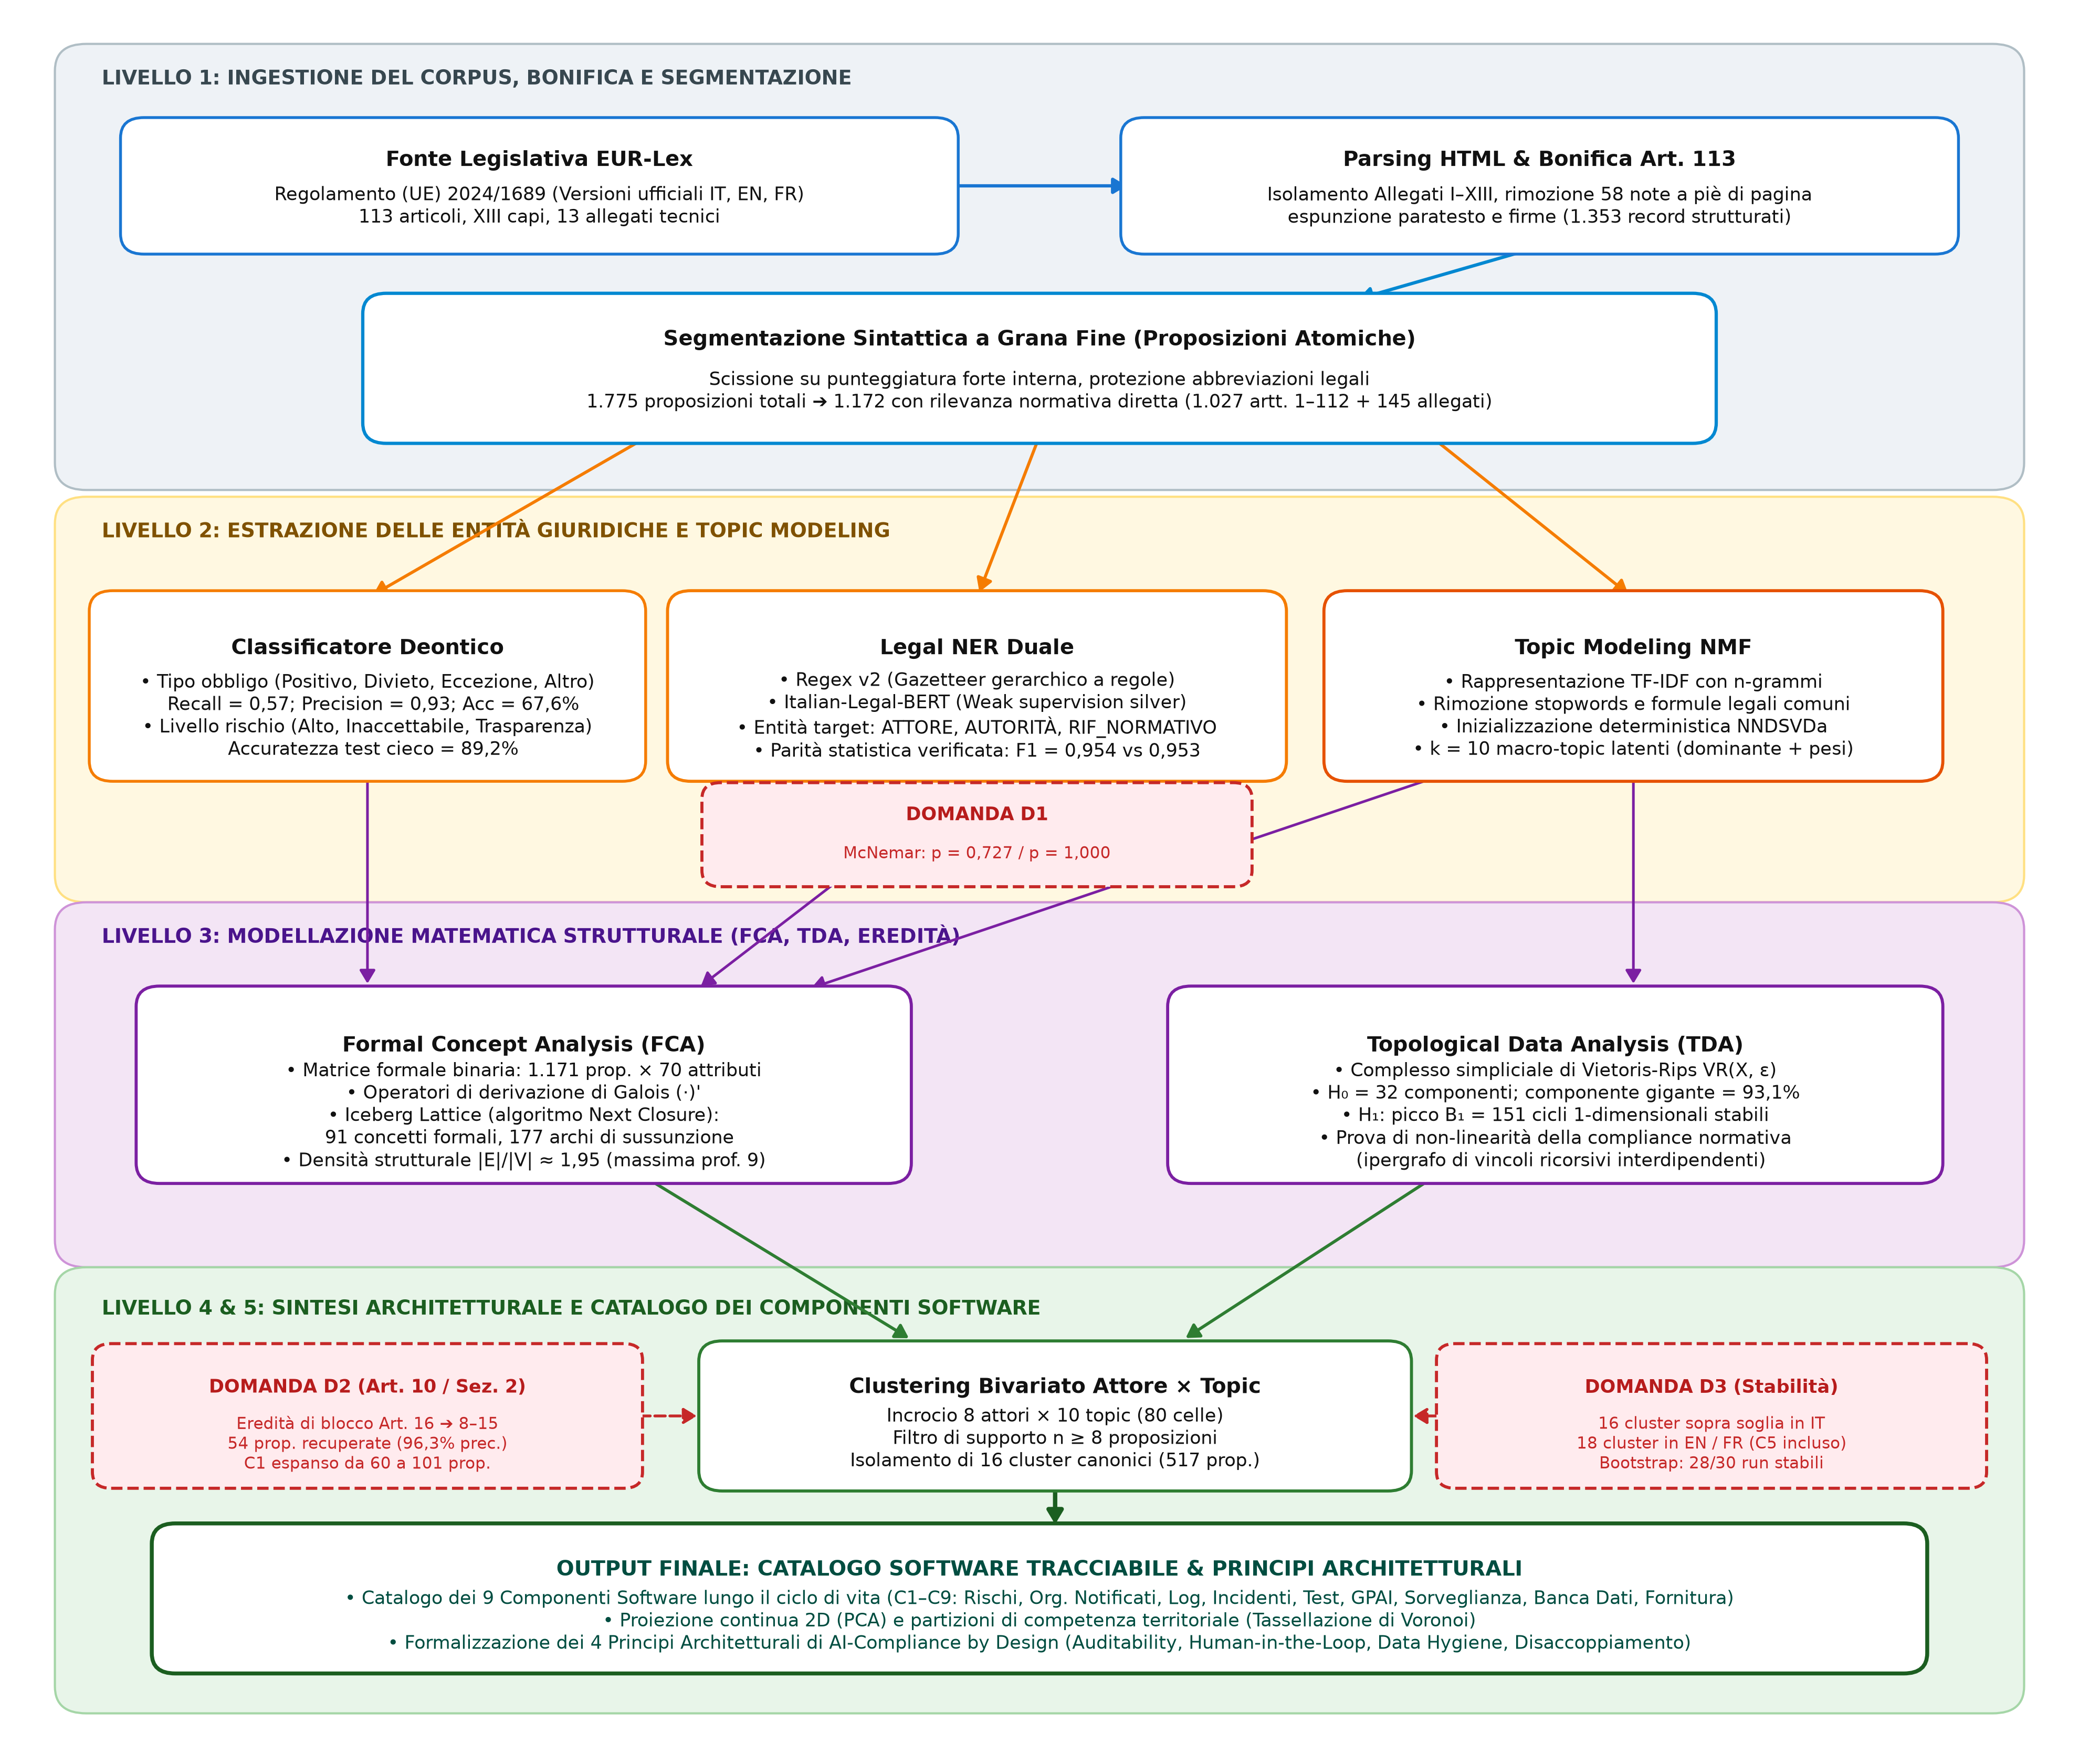
\includegraphics[width=0.8\linewidth]{pipeline_architettura.png}%
    }{%
        \fbox{\parbox[c][4cm][c]{0.8\linewidth}{\centering \texttt{[Immagine: pipeline\_architettura.png]}}}%
    }
    \caption[Architettura complessiva della pipeline computazionale]{Architettura tecnica end-to-end della pipeline computazionale a 5 livelli, con evidenziazione dei flussi di elaborazione e della collocazione delle tre domande di ricerca ($\mathcal{D}_1, \mathcal{D}_2, \mathcal{D}_3$).}
    \label{fig:placeholder}
\end{figure}

Il flusso informativo attraversa cinque stadi integrati:
\begin{enumerate}
    \item \textbf{Livello 1 --- Ingestione e Pre-processing}: acquisizione del testo HTML da EUR-Lex, disaccoppiamento degli allegati tecnici, rimozione del paratesto ed esecuzione della segmentazione in proposizioni atomiche;
    \item \textbf{Livello 2 --- Doppio binario NLP}: classificazione deterministica di categorie deontiche e livelli di rischio, affiancata dal Named Entity Recognition duale (\emph{Rules v2} vs \emph{Italian-Legal-BERT}), snodo in cui si colloca la domanda \textbf{$\mathcal{D}_1$};
    \item \textbf{Livello 3 --- Modellazione Matematica Strutturale}: estrazione non supervisionata dei 10 macro-topic via NMF, impiegati per l'analisi omologica multi-scala (TDA) e per la costruzione della matrice dei concetti formali (FCA);
    \item \textbf{Livello 4 --- Risoluzione degli Attori Impliciti}: superamento dell'impersonalità della Sezione 2 del Capo III mediante la regola formale di eredità dall'Articolo 16 agli Articoli 8--15, rispondendo alla domanda \textbf{$\mathcal{D}_2$};
    \item \textbf{Livello 5 --- Sintesi Architetturale e Catalogo Software}: incrocio bivariato Attore $\times$ Topic sopra soglia ($n \ge 8$) per isolare i cluster canonici (\textbf{$\mathcal{D}_3$}), loro proiezione spaziale e aggregazione nei 9 componenti software del catalogo architetturale.
\end{enumerate}

% -----------------------------------------------------------------------------
\section{Acquisizione, bonifica e granularità proposizionale}
\label{sec:acquisizione_bonifica}

Il corpus di riferimento è il testo consolidato del Regolamento (UE) 2024/1689 pubblicato nella Gazzetta Ufficiale dell'Unione Europea del 12 luglio 2024, scaricato direttamente da EUR-Lex (\texttt{ai\_act\_it.html}). La versione italiana costituisce l'asse principale di analisi, integrata dalle versioni ufficiali in lingua inglese (\texttt{ai\_act\_en.html}) e francese (\texttt{ai\_act\_fr.html}) per accertare la portabilità translinguistica dei metodi.

\paragraph{Perimetro del testo e bonifica degli allegati}
L'atto legislativo si compone di 113 articoli (distribuiti in XIII capi) e di 13 allegati tecnici. Nelle fasi preliminari della ricerca, il parser HTML inglobava impropriamente gli allegati e il paratesto finale all'interno dell'Articolo 113. 

La bonifica condotta dallo script \texttt{build\_norm\_sentence\_dataset.py} ha operato tre interventi correttivi:
\begin{enumerate}
    \item \textbf{Disaccoppiamento degli allegati}: assegnazione di un identificativo gerarchico dedicato a ciascun allegato (ad es.\ \texttt{AllIII\_par1\_a\_sent1});
    \item \textbf{Espunzione del paratesto}: rimozione completa delle 58 note bibliografiche a piè di pagina della Gazzetta Ufficiale (classe CSS \texttt{oj-note}) e della formula di chiusura (\texttt{oj-final});
    \item \textbf{Filtraggio dei metadati portale}: esclusione delle stringhe di servizio web (codici ELI, ISSN e menu EUR-Lex).
\end{enumerate}

Gli articoli 1--112 sono rimasti rigorosamente immutati in tutte e tre le lingue. Il dataset consolidato conta \textbf{1.353 record strutturati} (paragrafi e lettere) e \textbf{1.775 proposizioni atomiche}, di cui \textbf{1.172 a rilevanza normativa diretta} (\texttt{is\_normativa = True}), come riassunto nella Tabella~\ref{tab:statistiche_corpus}:

\begin{table}[H]
    \centering
    \small
    \caption[Statistiche del corpus prima e dopo la bonifica]{Statistiche del corpus normativo italiano prima e dopo la bonifica dell'Articolo 113 e degli allegati.}
    \label{tab:statistiche_corpus}
    \renewcommand{\arraystretch}{1.3}
    \begin{tabular}{l c c}
        \toprule
        \textbf{Livello del dato} & \textbf{Prima della bonifica} & \textbf{Corpus consolidato} \\
        \midrule
        Record strutturati (paragrafi e lettere) & 1.456 & \textbf{1.353} \\
        Proposizioni totali & 1.852 & \textbf{1.775} \\
        Proposizioni normative (\texttt{is\_normativa = True}) & 1.208 & \textbf{1.172} \\
        --- di cui negli allegati tecnici & \emph{(annidati in art.~113)} & \textbf{145} \\
        \bottomrule
    \end{tabular}
\end{table}

\paragraph{Segmentazione interna e scelta della granularità}
Ciascun record è segmentato in \textbf{proposizioni normative atomiche} combinando criteri sintattici ed elenchi di protezione:
\begin{itemize}
    \item Scissione su punteggiatura forte (punto, punto interrogativo, punto esclamativo) seguita da spazio e maiuscola;
    \item Protezione esplicita delle abbreviazioni legali ricorrenti (\emph{art.}, \emph{par.}, \emph{lett.}, \emph{n.}, \emph{nn.}, \emph{p.}, \emph{pp.}, \emph{v.});
    \item Scissione su punto e virgola quando separa statuizioni autonome all'interno dei medesimi commi;
    \item Eliminazione dei frammenti residui con meno di tre parole.
\end{itemize}

Dall'applicazione dello schema risultano 1.775 proposizioni atomiche da 1.318 record generativi (media di 1,35 proposizioni per record). 

La scelta di operare a livello di \textbf{proposizione} anziché di singola \textbf{clausola grammaticale} (soggetto-verbo-oggetto) risponde a tre vincoli per l'Ingegneria dei Requisiti:
\begin{enumerate}
    \item \emph{Preservazione del soggetto coordinato}: la coordinazione verbale (<<\emph{il fornitore redige\dots\ e conserva\dots}>>) omette il soggetto nella seconda clausola, generando proposizioni orfane;
    \item \emph{Integrità delle eccezioni}: isolare le subordinate condizionali (<<\emph{salvo che\dots}>>) trasformerebbe obblighi condizionati in vincoli assoluti;
    \item \emph{Robustezza sintattica}: i parser di dipendenze presentano elevata fragilità sui periodi normativi multilivello della legislazione europea.
\end{enumerate}

% -----------------------------------------------------------------------------
\section{Classificazione deontica e del livello di rischio}
\label{sec:classificazione_deontica_rischio}

Ciascuna proposizione è classificata sul proprio testo mediante regole deterministiche lungo due dimensioni ortogonali: la natura deontica del comando e il livello di rischio menzionato.

\paragraph{Gerarchia deontica e livelli di rischio}
La categoria deontica è determinata applicando una gerarchia di precedenza che assegna la prima etichetta riscontrata nel testo:
\begin{enumerate}
    \item \texttt{definizione}: enunciati definitori brevi contenenti locuzioni come \emph{si intende per}, \emph{designa} o il costrutto \texttt{<<termine>>: spiegazione};
    \item \texttt{divieto}: espressioni negative perentorie quali \emph{è vietato}, \emph{non deve}, \emph{non possono};
    \item \texttt{eccezione}: clausole limitative o derogatorie (\emph{tuttavia}, \emph{salvo}, \emph{a meno che}, \emph{non si applica});
    \item \texttt{obbligo\_positivo}: costrutti di dovere forte (\emph{deve}, \emph{è tenuto a}) o verbi all'indicativo presente utilizzati in funzione precettiva (\emph{garantisce}, \emph{redige}, \emph{adotta});
    \item \texttt{altro}: disposizioni descrittive, procedurali o definitorie ampie.
\end{enumerate}
La precedenza dell'eccezione rispetto all'obbligo assicura che clausole complesse (<<\emph{i fornitori adottano misure\dots\ a meno che\dots}>>) siano etichettate in base alla condizione limitativa più specifica.

Il \texttt{livello\_rischio} isola le menzioni esplicite nel testo: \texttt{high} (sistemi ad alto rischio o Allegato III), \texttt{unacceptable} (pratiche vietate ex Art.~5), \texttt{transparency} (obblighi di trasparenza ex Art.~50), oppure \texttt{none} (1.398 proposizioni, in cui il rischio è implicito nella collocazione sistematica).

\paragraph{Estensione multilingue (Inglese e Francese)}
La classificazione è stata replicata nelle versioni in lingua inglese (\texttt{build\_dataset\_en.py}) e francese (\texttt{build\_dataset\_fr.py}), gestendo le specificità sintattiche delle traduzioni ufficiali: l'inglese adotta il modale <<\emph{shall}>> (con filtri di esclusione per formule procedurali dell'atto), mentre il francese adotta la formula \texttt{<<terme>>,} con la virgola, la marcatura <<\emph{Article premier}>> e costruzioni passive all'indicativo (\emph{est/sont + participio}).

La Tabella~\ref{tab:distribuzione_deontica} confronta la distribuzione delle classi deontiche estratte nelle tre lingue:

\begin{table}[H]
    \centering
    \small
    \renewcommand{\arraystretch}{1.3}
    \begin{tabular}{l c c c}
        \toprule
        \textbf{Categoria deontica} & \textbf{Italiano (IT)} & \textbf{Inglese (EN)} & \textbf{Francese (FR)} \\
        \midrule
        Obbligo positivo & 208 (11,7\%) & 488 (27,5\%) & 238 (13,4\%) \\
        Divieto & 17 (1,0\%) & 18 (1,0\%) & 19 (1,1\%) \\
        Eccezione & 68 (3,8\%) & 62 (3,5\%) & 55 (3,1\%) \\
        Definizione & 43 (2,4\%) & 42 (2,4\%) & 42 (2,4\%) \\
        Altro (descrizioni/procedure) & 1.441 (81,1\%) & 1.167 (65,7\%) & 1.423 (80,1\%) \\
        \midrule
        \textbf{Totale proposizioni} & \textbf{1.777} & \textbf{1.777} & \textbf{1.777} \\
        \bottomrule
    \end{tabular}
    \caption[Distribuzione comparativa delle classi deontiche]{Distribuzione delle classi deontiche estratte nelle tre versioni ufficiali dell'AI Act.}
    \label{tab:distribuzione_deontica}
\end{table}

% -----------------------------------------------------------------------------
\section{Riconoscimento delle entità giuridiche (Legal NER)}
\label{sec:ner_metodologia}

Il Named Entity Recognition estrae le tre classi fondamentali di entità nel testo normativo:
\begin{enumerate}
    \item \texttt{ATTORE}: i soggetti destinatari di doveri o ruoli (fornitore, deployer, importatore, distributore, rappresentante autorizzato, operatore);
    \item \texttt{AUTORITA}: le istituzioni pubbliche e gli organismi di controllo (Ufficio per l'IA, Commissione, autorità di vigilanza del mercato, organismo notificato);
    \item \texttt{RIF\_NORMATIVO}: i riferimenti formali a componenti del Regolamento o ad altri atti legislativi (articoli, paragrafi, allegati, direttive, regolamenti).
\end{enumerate}

\paragraph{Approccio simbolico a regole (Rules v2)}
Il motore a regole (\texttt{ner\_rule\_based.py}) opera mediante espressioni regolari e gazetteer calibrati sulle convenzioni tipografiche di EUR-Lex:
\begin{itemize}
    \item \textbf{Risoluzione delle sovrapposizioni}: la funzione \texttt{resolve\_overlaps} assegna priorità allo span più lungo e specifico (ad es.\ <<\emph{organismo di valutazione della conformità}>> rispetto a <<\emph{organismo}>>);
    \item \textbf{Forme composite e qualificatori}: pattern dedicati intercettano ruoli qualificati (<<\emph{fornitori di modelli di IA per finalità generali}>>) e citazioni articolate (<<\emph{articolo 9, paragrafo 1, lettera a)}>>);
    \item \textbf{Normalizzazione canonica}: ciascuna menzione viene ricondotta alla sua etichetta di dominio (ad es.\ <<\emph{deployers}>> ed <<\emph{utilizzatori}>> convergono a \texttt{deployer}), alimentando il contesto formale binario.
\end{itemize}

\paragraph{Modelli linguistici Transformer di dominio}
Parallelamente alle regole, sono stati addestrati tre modelli Transformer pre-addestrati sul linguaggio giuridico delle rispettive lingue:
\begin{itemize}
    \item \textbf{Italiano}: \texttt{dlicari/Italian-Legal-BERT} ($\approx 110\text{M}$ parametri; Licari et al., 2022);
    \item \textbf{Inglese}: \texttt{nlpaueb/legal-bert-base-uncased} ($110\text{M}$ parametri; Chalkidis et al., 2020);
    \item \textbf{Francese}: \texttt{dascim/juribert-base} (\emph{JuriBERT}, $\approx 100\text{M}$ parametri; Douka et al., 2021).
\end{itemize}

Ciascun modello adotta una testa di token classification con schema IOB2 sulle tre classi. L'addestramento è avvenuto con \textbf{supervisione debole} (\emph{silver labels}) generate automaticamente dalle regole v2 su circa 940 proposizioni non utilizzate nei test ciechi. Questo impianto duale consente il confronto formale richiesto dalla domanda $\mathcal{D}_1$.

% -----------------------------------------------------------------------------
\section{Modellazione semantica con Non-negative Matrix Factorization (NMF)}
\label{sec:nmf_metodologia}

Per estrarre i temi latenti dell'AI Act in modo trasparente e interpretabile, la pipeline adotta la \textbf{Non-negative Matrix Factorization (NMF)} (Lee e Seung, 1999). A differenza dei metodi generativi probabilistici (LDA), NMF produce una rappresentazione a parti sparse (\emph{part-based}) che evidenzia blocchi lessicali ben definiti.

\subsection*{Formulazione matematica}
Sia $V \in \mathbb{R}_{\ge 0}^{N \times M}$ la matrice termine-documento non negativa ($N = 1.171$ proposizioni normative operative e $M$ termini distintivi), pesata mediante metrica \textbf{TF-IDF}:
\begin{equation}
    \text{TF-IDF}(t, d, D) = \text{TF}(t, d) \times \left(1 + \ln\frac{1 + |D|}{1 + |\{d' \in D : t \in d'\}|}\right)
\end{equation}
La matrice include unigrammi e bigrammi (frequenza minima su almeno tre proposizioni), previa rimozione delle stopword della lingua italiana e del lessico procedurale comunitario (<<\emph{articolo}>>, <<\emph{comma}>>, <<\emph{regolamento}>>, <<\emph{disposizioni}>>).

NMF fattorizza $V$ nel prodotto di due matrici a rango ridotto $k \ll \min(N, M)$:
\begin{equation}
    V \approx W \times H
\end{equation}
dove $W \in \mathbb{R}_{\ge 0}^{N \times k}$ rappresenta i pesi di assegnazione documento--tema e $H \in \mathbb{R}_{\ge 0}^{k \times M}$ i profili lessicali dei temi. L'ottimizzazione minimizza la norma di Frobenius con regolarizzazione L1/L2:
\begin{equation}
    \min_{W \ge 0, H \ge 0} \frac{1}{2} \|V - W H\|_F^2 + \alpha \rho (\|W\|_1 + \|H\|_1) + \frac{\alpha(1-\rho)}{2} (\|W\|_F^2 + \|H\|_F^2)
\end{equation}

\subsection*{Determinismo e selezione di $k$}
Per eliminare la variabilità stocastica dell'inizializzazione casuale, la pipeline impiega l'algoritmo deterministico \textbf{NNDSVDa} (Boutsidis e Gallopoulos, 2008), fondato sui vettori singolari positivi della matrice SVD. Fissato \textbf{$k = 10$}, a ogni proposizione $i$ viene associato il \textbf{tema dominante} $t^*(i) = \arg\max_j W_{i, j}$.

% -----------------------------------------------------------------------------
\section{Analisi topologica dei dati (TDA)}
\label{sec:tda_metodologia}

Mentre NMF riduce ciascuna proposizione a un singolo tema dominante forzando una partizione discreta, la \textbf{Topological Data Analysis (TDA)} (Carlsson, 2009; Edelsbrunner e Harer, 2010) caratterizza la geometria intrinseca dello spazio normativo sull'intero vettore continuo dei pesi tematici.

\subsection*{Spazio metrico e complessi di Vietoris-Rips}
Ciascuna proposizione $i \in G$ è descritta dal vettore normalizzato dei pesi tematici $w_i = (W_{i, 1}, \dots, W_{i, 10}) \in \mathbb{R}^{10}$, dotato della metrica del coseno:
\begin{equation}
    d_{\cos}(w_i, w_j) = 1 - \frac{w_i \cdot w_j}{\|w_i\|_2 \|w_j\|_2} \in [0, 1]
\end{equation}

Al variare continuo del raggio di prossimità $\epsilon \ge 0$, si costruisce la filtrazione simpliciale di \textbf{Vietoris-Rips} $\text{VR}(X, \epsilon)$, i cui vertici corrispondono alle 1.171 proposizioni e i cui spigoli uniscono coppie aventi distanza $d_{\cos}(w_i, w_j) \le \epsilon$.

\subsection*{Persistenza omologica}
L'omologia persistente traccia la comparsa e la scomparsa dei generatori topologici lungo la filtrazione:
\begin{itemize}
    \item \textbf{Gruppo $H_0$ (Numero di Betti $\beta_0(\epsilon)$)}: quantifica il numero di \textbf{componenti connesse} indipendenti a raggio $\epsilon$, permettendo di verificare se il corpus si frammenti in blocchi semantici isolati o converga in una macro-componente connessa;
    \item \textbf{Gruppo $H_1$ (Numero di Betti $\beta_1(\epsilon)$)}: quantifica i \textbf{cicli unidimensionali persistenti} (anelli chiusi di vincoli non collassabili). Un elevato numero di cicli $\beta_1$ fornisce la prova matematica che le prescrizioni dell'atto formano un reticolo di vincoli interdipendenti e non lineari.
\end{itemize}

% -----------------------------------------------------------------------------
\section{Analisi formale dei concetti (FCA)}
\label{sec:fca_metodologia}

La \textbf{Formal Concept Analysis (FCA)} (Ganter e Wille, 1999) fornisce lo strumento algebrico per derivare gerarchie concettuali esatte dalla matrice delle co-occorrenze tra proposizioni ed entità.

\subsection*{Il contesto formale binario $(G, M, I)$}
Il contesto formale è una tripla $\mathbb{K} = (G, M, I)$, dove:
\begin{itemize}
    \item $G$ è l'insieme di \textbf{1.171 proposizioni normative};
    \item $M$ è l'insieme di \textbf{70 attributi binari}: 10 temi NMF (\texttt{topic\_0}--\texttt{topic\_9}), 3 flag di presenza generica (\texttt{has\_attore}, \texttt{has\_autorita}, \texttt{has\_rif\_normativo}), 17 attori regolati, 19 autorità pubbliche, 12 rinvii normativi espliciti, 5 classi deontiche e 4 livelli di rischio;
    \item $I \subseteq G \times M$ è la relazione binaria indicante il possesso dell'attributo da parte della proposizione.
\end{itemize}

\subsection*{Connessione di Galois e reticoli Iceberg}
Gli operatori di derivazione di Galois associano a ogni sottoinsieme di oggetti $A \subseteq G$ e attributi $B \subseteq M$:
\begin{equation}
    A' = \{m \in M \mid \forall g \in A, \, (g, m) \in I\}, \qquad B' = \{g \in G \mid \forall m \in B, \, (g, m) \in I\}
\end{equation}
Un \textbf{concetto formale} è una coppia $(A, B)$ tale che $A' = B$ e $B' = A$, dove $A$ è l'estensione e $B$ l'intensione. L'ordinamento parziale per sussunzione concettuale:
\begin{equation}
    (A_1, B_1) \le (A_2, B_2) \iff A_1 \subseteq A_2 \quad (\iff B_2 \subseteq B_1)
\end{equation}
definisce un reticolo completo generato mediante l'algoritmo \textbf{Next Closure} (Ganter, 2010). Per prevenire l'esplosione combinatoria e isolare i nuclei informativi rilevanti, la pipeline estrae l'\textbf{Iceberg Lattice} (Stumme et al., 2002), selezionando i soli concetti con supporto $|A| \ge \text{minsup}$.

% -----------------------------------------------------------------------------
\section{Sintesi dei cluster bivariati e catalogo architetturale}
\label{sec:sintesi_cluster_metodologia}

La fase conclusiva della pipeline formalizza il passaggio dal piano descrittivo a quello architetturale attraverso tre procedure metodologiche:

\subsection*{1. Criterio di clustering bivariato Attore $\times$ Topic (Risposta a $\mathcal{D}_3$)}
La combinazione tra gli attori regolati e i 10 macro-topic NMF produce una griglia di co-occorrenza. Per ogni coppia $(a, t)$, il supporto normativo è definito come:
\begin{equation}
    \text{Supporto}(a, t) = |\{g \in G \mid g \in \text{Attore}(a) \land g \in \text{Topic}(t) \land \texttt{tipo\_obbligo}(g) \ne \text{<<definizione>>}\}|
\end{equation}
Fissata una soglia minima di robustezza $\text{Supporto} \ge 8$ proposizioni, si isolano i \textbf{cluster canonici sopra soglia}, garantendo che ciascun raggruppamento poggi su una base probatoria consistente.

\subsection*{2. Regola di eredità strutturale per la Sezione 2 (Risposta a $\mathcal{D}_2$)}
Per superare l'impersonalità linguistica della Sezione 2 del Capo III (Artt.~8--15), i cui requisiti tecnici non citano attori espliciti nel testo, la metodologia applica una regola formale di derivazione di contesto basata sul rimando dell'Articolo~16:
\begin{equation}
    \forall g \in \text{Sezione 2} : \texttt{has\_attore}(g) = 0 \implies \texttt{attore}(g) \leftarrow \text{<<fornitore>>}
\end{equation}
Tale regola ascrive oggettivamente al fornitore i requisiti di sistema (Data Governance, Logging, Human Oversight), recuperando le proposizioni orfane.

\subsection*{3. Strutturazione dei 9 componenti software del catalogo}
I cluster bivariati stabili vengono infine mappati nei \textbf{9 componenti software del catalogo architetturale} (C1--C9), articolati lungo le quattro fasi del ciclo di vita del sistema di IA:
\begin{enumerate}
    \item \emph{Sviluppo e classificazione}: C1 (Vaglio e governance del rischio), C5 (Governance test in condizioni reali), C6 (Modulo conformità GPAI);
    \item \emph{Valutazione della conformità}: C2 (Interfaccia organismo notificato), C3 (Registro documentale e archivio);
    \item \emph{Immissione sul mercato}: C8 (Registrazione banca dati UE), C9 (Verifica conformità supply chain);
    \item \emph{Monitoraggio post-market}: C4 (Pipeline segnalazione incidenti), C7 (Sorveglianza umana e controlli).
\end{enumerate}

La quantificazione sperimentale dei cluster, la proiezione spaziale di Voronoi e le verifiche di robustezza costituiscono l'oggetto del Capitolo 4.

\clearpage

% =============================================================================
% CAPITOLO 4
% =============================================================================

\chapter{Risultati sperimentali ed evidenze empiriche}
Il presente capitolo espone in modo rigoroso, quantitativo e asettico l'intero corpus dei risultati sperimentali scaturiti dall'esecuzione della pipeline computazionale descritta nel \cref{cap:metodologia}. Si presentano la caratterizzazione statistica del corpus normativo, i protocolli ciechi di validazione dei classificatori e del Named Entity Recognition con i rispettivi test di significatività per rispondere alla domanda di ricerca $\mathcal{D}_1$, i riscontri di Topic Modeling (NMF), analisi topologica (TDA) e reticoli formali (FCA), fino alla derivazione \emph{bottom-up} del catalogo dei 9 componenti software, integrando la quantificazione dell'eredità per l'Articolo 10 e la Sezione 2 (risposta a $\mathcal{D}_2$), le proiezioni spaziali dei cluster e le verifiche di robustezza multilingue e parametrica 
(risposta a $\mathcal{D}_3$).


\section{Caratterizzazione del dataset e segmentazione sintattica}
\label{sec:risultati_dataset}

Il corpus operativo consolidato del Regolamento (UE) 2024/1689 scaricato da EUR-Lex, a seguito della bonifica dell'Articolo 113 e dello scorporo del paratesto con le 58 note bibliografiche, è cosi strutturato:

\begin{itemize}
    \item \textbf{\num{1353} record strutturati} originari (commi e punti elenco dell'atto);
    \item \textbf{\num{1775} proposizioni atomiche compulsive} (contro le \num{1852} grezze pre-bonifica);
    \item \textbf{\num{1172} proposizioni con rilevanza normativa diretta} (\campo{is_normativa = True}): \num{1027} negli articoli 1--112, 145 negli allegati tecnici (I--XIII) e 1 di chiusura nell'Art.~113;
    \item \textbf{\num{1171}proposizioni operative} impiegate stabilmente nelle matrici di modellazione semantica (NMF, TDA e FCA), previa rimozione di un singolo record privo di contenuto lessicale autonomo.
\end{itemize}

L'analisi distribuzionale sulle \num{1172} proposizioni normative evidenzia la forte asimmetria nella redazione del testo comunitario (\cref{tab:distribuzione_corpus}): solo il \SI{17,7}{\percent} esprime un \campo{obbligo_positivo} esplicito, mentre il \SI{72,0}{\percent} ricorre a forme descrittive o procedimentali all'indicativo presente (\campo{altro}). Analogamente, il \SI{69,8}{\percent} delle norme non reca menzione lessicale diretta del livello di rischio, concentrando i requisiti qualificati sul sottoinsieme \campo{alto_rischio} (\SI{23,1}{\percent}, 271 proposizioni).


\begin{table}[htbp]
  \centering
  \small
  \caption[Distribuzione delle modalità deontiche e del rischio]{Distribuzione delle frequenze delle proposizioni normative ($N=\num{1172}$).}
  \label{tab:distribuzione_corpus}
  \begin{tabular}{llr llr}
    \toprule
    \textbf{Tipo obbligo} & \textbf{Prop.} & \textbf{\%} & \textbf{Livello rischio} & \textbf{Prop.} & \textbf{\%} \\
    \midrule
    \campo{obbligo_positivo} & 208 & \SI{17,7}{\percent} & \campo{alto_rischio} & 271 & \SI{23,1}{\percent} \\
    \campo{divieto} & 42 & \SI{3,6}{\percent} & \campo{trasparenza / limitato} & 45 & \SI{3,8}{\percent} \\
    \campo{definizione} & 43 & \SI{3,7}{\percent} & \campo{rischio_inaccettabile} & 38 & \SI{3,2}{\percent} \\
    \campo{eccezione} & 35 & \SI{3,0}{\percent} & \campo{nessuna menzione} & 818 & \SI{69,8}{\percent} \\
    \campo{altro} (indicativo) & 844 & \SI{72,0}{\percent} & & & \\
    \midrule
    \textbf{Totale normativo} & \textbf{\num{1172}} & \SI{100,0}{\percent} & \textbf{Totale normativo} & \textbf{\num{1172}} & \SI{100,0}{\percent} \\
    \bottomrule
  \end{tabular}
\end{table}
%_____________
\section{Validazione empirica della classificazione e del NER Domanda \texorpdfstring{$\mathcal{D}_1$}{D1})}
\label{sec:risultati_ner_validazione}

Tutte le metriche di prestazione del Named Entity Recognition sono calcolate in modalità \textbf{strict}: un'entità è corretta se e solo se sia la classe che l'esatto intervallo di caratteri (\emph{span}) coincidono al 100\% con il gold standard annotato a mano.

\subsection{Validazione del classificatore delle proposizioni}
Il classificatore deterministico a regole per \textit{tipo\_obbligo} e \textit{livello\_rischio} è stato valutato confrontando la prima stima di sviluppo con un protocollo di validazione cieco e non circolare.

\begin{itemize}
    \item \textbf{Prima stima (circolare, 194 proposizioni)}: accuratezza apparente del \num{98,27}\% su \textit{tipo\_obbligo} e del \num{100}\% su \textit{livello\_rischio}. L'ispezione metodologica ha rilevato che il 43\% degli obblighi positivi era catturato da verbi introdotti esaminando il campione stesso.
    \item \textbf{Stima indipendente e cieca (49 proposizioni non viste, regole congelate}:
    \begin{itemize}
        \item Accuratezza su \textit{tipo\_obbligo} : 67,6\% (precisione 0,93, ma recall a 0,57 sull'obbligo positivo per l'impossibilità di enumerare tutte le forme all'indicativo deontico);
        \item Accuratezza su \textit{livello\_rischio}: 89,2\%.
    \end{itemize}
\end{itemize}

\subsection{Protocollo a round ciechi e test di McNemar (Risposta a \texorpdfstring{$\mathcal{D}_1$}{D1})}
Il riconoscimento delle entità giuridiche (\campo{ATTORE}, \campo{AUTORITA}, \campo{RIF_NORMATIVO}) è stato sviluppato e validato mediante quattro round progressivi:
\begin{itemize}
  \item \textbf{Round 1--3 (Raffinamento e diagnosi)}: l'annotazione cieca (Round 2, 60 proposizioni) ha evidenziato bias di ancoraggio cognitivo e isolato 4 lacune sintattiche del gazetteer; corrette le regole (Round 3, 60 proposizioni), il sistema simbolico è salito a $F_1 = \num{0,87}$ (richiamo su \campo{ATTORE} a \num{0,96}).
  \item \textbf{Diagnosi dei 44 errori comuni con Legal-BERT v1}: l'analisi appaiata ha rivelato che nel 75\% dei casi (33 su 44) BERT sbagliava esattamente come il gazetteer, e che 30 errori derivavano da bug formali delle regole (auto-riferimento \enquote{\emph{presente articolo}}, virgole nei rinvii). Rilasciate le regole \textbf{v2} e riaddestrato Legal-BERT sulle nuove silver labels, si è proceduto alla valutazione finale.
  \item \textbf{Benchmark finale}: condotto su un pool congelato di \textbf{220 proposizioni indipendenti (379 entità gold)} e confermato da un quarto round cieco puro (60 proposizioni mai viste, 88 entità gold; \cref{tab:ner_mcnemar}).
\end{itemize}

\begin{table}[htbp]
  \centering
  \small
  \caption[Metriche comparative definitive dei sistemi NER e Test di McNemar]{Metriche comparative definitive strict dei sistemi NER e test di significatività appaiato di McNemar (Risposta a $\mathcal{D}_1$).}
  \label{tab:ner_mcnemar}
  \begin{tabular}{llrrrcc}
    \toprule
    \textbf{Campione di test} & \textbf{Sistema NER} & \textbf{Prec.} & \textbf{Rec.} & \textbf{F1} & \textbf{Discordanze} & \textbf{p-value (McNemar)} \\
    \midrule
    \textbf{Pooled pulito} & \textbf{Rules v2} & \num{0,958} & \num{0,950} & \textbf{\num{0,954}} & \multirow{2}{*}{3 vs 5} & \multirow{2}{*}{$p = \num{0,727}$ (Parità)} \\
    (379 entità gold) & \textbf{Legal-BERT v2} & \num{0,955} & \num{0,951} & \textbf{\num{0,953}} & & \\
    & spaCy generalista & \num{0,281} & \num{0,239} & \num{0,258} & --- & --- \\
    \midrule
    \textbf{Round 4 cieco} & \textbf{Rules v2} & \num{0,926} & \num{0,916} & \textbf{\num{0,921}} & \multirow{2}{*}{1 vs 1} & \multirow{2}{*}{$p = \num{1,000}$ (Parità)} \\
    (88 entità gold) & \textbf{Legal-BERT v2} & \num{0,920} & \num{0,912} & \textbf{\num{0,916}} & & \\
    & spaCy generalista & \num{0,238} & \num{0,211} & \num{0,223} & --- & --- \\
    \bottomrule
  \end{tabular}
\end{table}

Il test non parametrico di McNemar certifica la \textbf{perfetta parità statistica} ($p=\num{0,727}$ sul pooled, $p=\num{1,000}$ al Round 4 cieco). Per verificare se tale equivalenza derivasse unicamente dall'addestramento su silver labels, è stato condotto un esperimento controllato con \textbf{5-fold Cross-Validation} addestrando Legal-BERT esclusivamente su 309 proposizioni annotate a mano (591 entità gold; \cref{tab:bert_controllo}): da solo, LegalBERT crolla a $F_1 = \num{0,821}$ ($p<\num{0,001}$), mentre con pre-addestramento debole sulle regole risale a \num{0,940} allineandosi alla baseline simbolica (\num{0,946}).

\begin{table}[htbp]
  \centering
  \small
  \caption[Confronto 5-fold Cross-Validation tra regimi di supervisione]{Confronto su 5-fold Cross-Validation tra regimi di supervisione forte e debole per Legal-BERT.}
  \label{tab:bert_controllo}
  \begin{tabular}{p{5.5cm} c c p{4.2cm}}
    \toprule
    \textbf{Configurazione sperimentale} & \textbf{Round 4 F1} & \textbf{5-fold CV F1} & \textbf{Esito metodologico} \\
    \midrule
    \textbf{A $\cdot$ Rules v2} (baseline deterministica) & \num{0,921} & \textbf{\num{0,946}} & Riferimento simbolico \\
    \textbf{B $\cdot$ Legal-BERT v2} (silver labels) & \num{0,916} & \num{0,942} & Parità con il maestro ($p > \num{0,50}$) \\
    \textbf{C $\cdot$ Legal-BERT sole note umane} & \num{0,857} & \textbf{\num{0,821}} & Collasso dati ($p < \num{0,001}$) \\
    \textbf{D $\cdot$ Legal-BERT silver + umane} & \textbf{\num{0,927}} & \num{0,940} & Parità asintotica con le regole \\
    \bottomrule
  \end{tabular}
\end{table}


%____________

\section{Risultati di modellazione semantica, topologica e concettuale}
\label{sec: risultati_semantica_topologica}

\subsection{Topic Modeling con NMF e Analisi Topologica (TDA)}
La decomposizione NMF deterministica ($k=10$, NNDSVDa) sulle \num{1171} proposizioni normative estrae 10 macro-temi latenti coesi (\cref{nmf_topics}), dominati dai requisiti tecnici per l'alto rischio (Topic 2, 242 prop.), adempimenti del fornitore (Topic 5, 146 prop.), produce di conformità (Topic 9, 133 prop.) e modelli GPAI (Topic 1, 122 prop.).

%\clearpage
\begin{table}[htbp]
  \centering
  \small
  \caption[I 10 macro-topic latenti estratti con NMF]{I 10 macro-topic latenti estratti con NMF ($k=10$) sul corpus consolidato.}
  \label{tab:nmf_topics}
  \begin{tabularx}{\textwidth}{c l X r}
    \toprule
    \textbf{Id} & \textbf{Termini rappresentativi} & \textbf{Nucleo concettuale} & \textbf{Prop.} \\
    \midrule
    \textbf{0} & mercato / vigilanza / vigilanza mercato & Vigilanza del mercato, notifiche e salvaguardia & 65 \\
    \textbf{1} & generali / finalità generali / finalità & Modelli GPAI e rischio sistemico & 122 \\
    \textbf{2} & rischio / alto rischio / alto & Requisiti tecnici dei sistemi ad alto rischio & 242 \\
    \textbf{3} & consiglio / europeo / parlamento & Rinvii ad altri atti normativi UE (Allegati I e X) & 46 \\
    \textbf{4} & organismo / notificato / org. notificato & Organismi notificati e requisiti CAB (Allegato VII) & 100 \\
    \textbf{5} & fornitore / dati / rappresentante & Dati da registrare, rappresentanti autorizzati, test & 146 \\
    \textbf{6} & competenti / autorità nazionali & Sandbox regolamentari e autorità nazionali & 111 \\
    \textbf{7} & atti / tiene / tiene conto & Atti delegati ed esecuzione & 82 \\
    \textbf{8} & membri / stati membri / stati & Cooperazione tra Stati membri e Commissione & 124 \\
    \textbf{9} & conformità / valutazione / valutazione conf. & Procedure formali di valutazione della conformità & 133 \\
    \midrule
    & & \textbf{Totale proposizioni analizzate} & \textbf{\num{1171}} \\
    \bottomrule
  \end{tabularx}
\end{table}

L'omologia persistente (Vietoris-Rips in $\mathbb{R}^{10}$, metrica del coseno, grafo $k$-NN con $k=18$) conferma la natura reticolare e non sequenziale del testo normativo (\cref{fig:tda_complessiva}):
\begin{enumerate}
  \item A soglia di stabilità ($\epsilon = \num{0,0897}$), una singola macro-componente in $H_0$ raggruppa \textbf{\num{1090} proposizioni su \num{1171} (il \SI{93,1}{\percent} del corpus)}, provando l'assenza di fratture o partizioni disgiunte a priori nel dettato comunitario;
  \item La curva dei numeri di Betti $\beta_1$ evidenzia un picco di \textbf{151 cicli semantici indipendenti} persistenti a $\epsilon = \num{0,1053}$, che quantificano geometricamente i vincoli incrociati di rinvio e correlazione tra obblighi tecnici.
\end{enumerate}

\begin{figure}[htbp]
  \centering
  \begin{subfigure}[b]{0.48\textwidth}
    \centering
    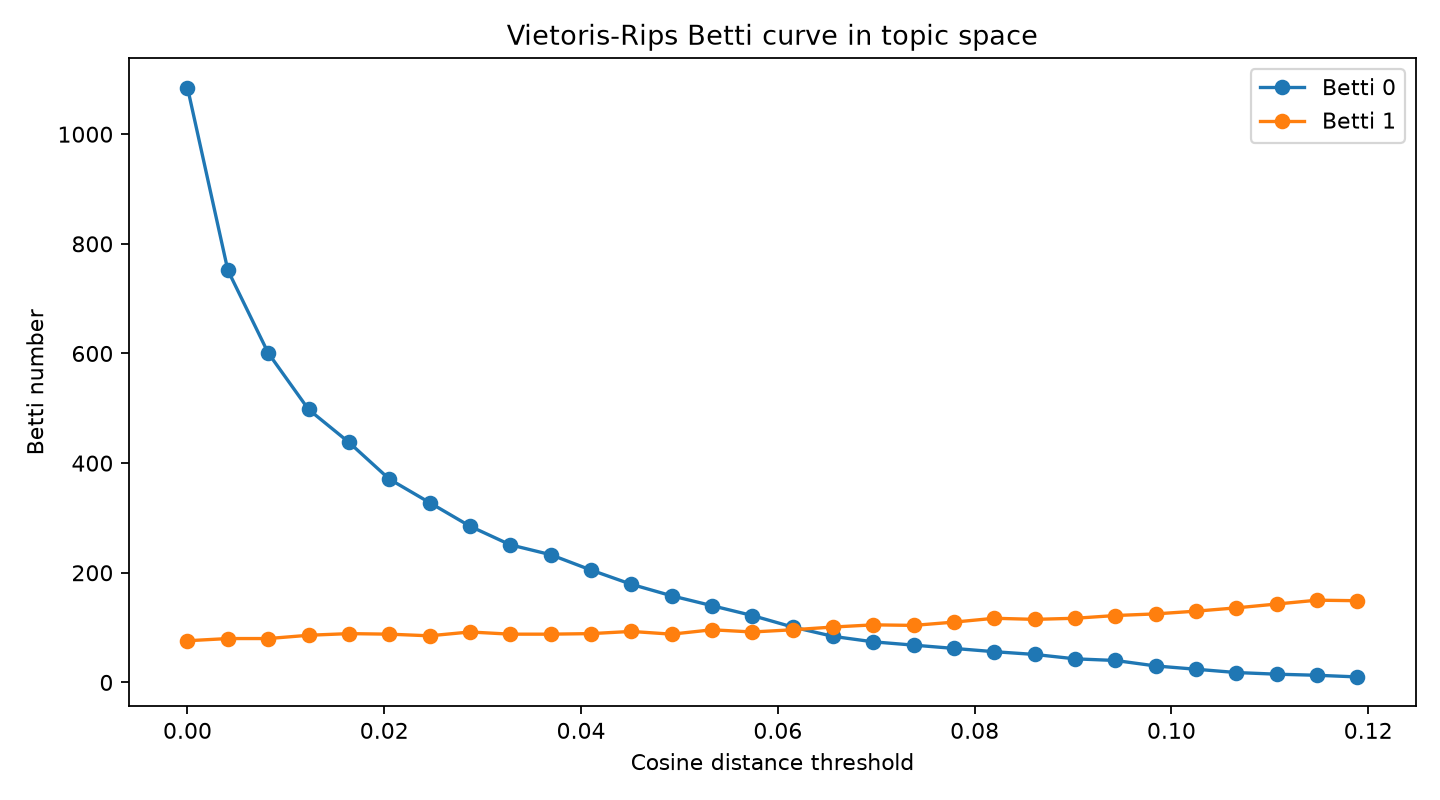
\includegraphics[width=\textwidth]{tda_betti_curve}
    \caption{Curve dei numeri di Betti $\beta_0$ e $\beta_1$ al variare di $\epsilon$.}
    \label{fig:tda_betti}
  \end{subfigure}
  \hfill
  \begin{subfigure}[b]{0.48\textwidth}
    \centering
    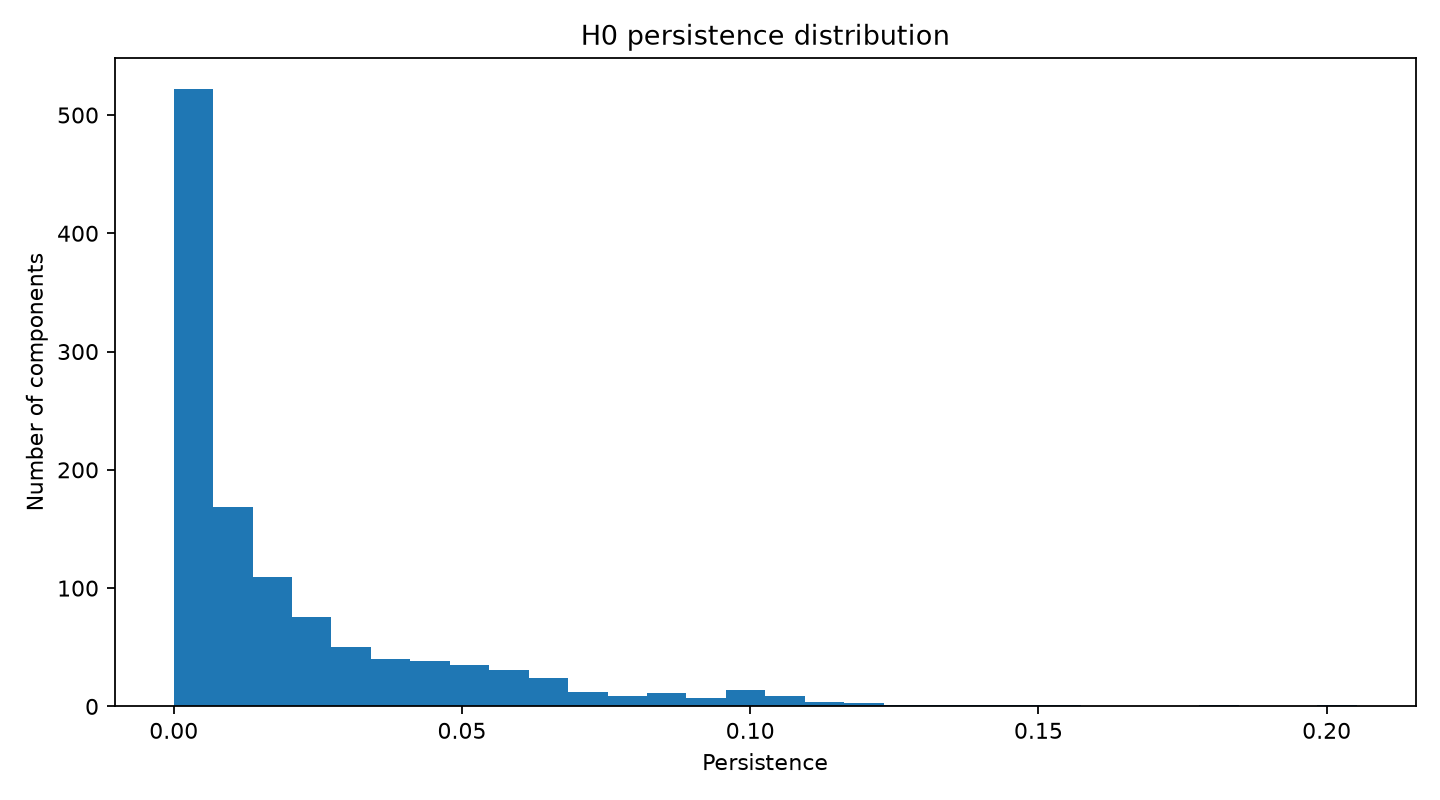
\includegraphics[width=\textwidth]{tda_h0_persistence.png}
    \caption{Diagramma di persistenza $H_0$ (fusione componente gigante).}
    \label{fig:tda_persistence}
  \end{subfigure}
  \caption[Analisi topologica dei dati dell'AI Act]{Risultati dell'Analisi Topologica dei Dati (TDA) sul corpus normativo: evidenza empirica della componente gigante e dei 151 cicli semantici persistenti.}
  \label{fig:tda_complessiva}
\end{figure}

\subsection{Rappresentazione concettuale mediante FCA}
\label{sec:risultati_fca}
La Formal Concept Analysis sulla matrice binaria $1171 \times70$ (densità \SI{8,2}{\percent}) produce mediante \emph{Nex Closure} un reticolo globale di \num{3696} concetti formali e \num{12576} archi. L'estrazione dell'\emph{Iceberg Lattice} (supporto $\ge 80$ proposizioni, $\approx \SI{7}{\percent}$) isola \textbf{91 concetti formali e 177 formali e 177 archi} su 4 livelli di sussunzione. Il concetto cardine di Livelo 1 è proprio \campo{has_attore} (549 proposizioni attive), confermando sul piano algebrico che l'attore giuricico costituisce il discriminante primario per strutturare la conformità.

%______

\subsection{Derivazione dei componenti, eredità e stabilità \texorpdfstring{$\mathcal{D}_2$}{D2} e \texorpdfstring{$\mathcal{D}_3$}{D3})}
\label{sec:risultati_componenti_stabilità}

\subsection{Derivazione dei 16 cluster bivariati e catalogo dei 9 componenti software} 
L'intersezione tra i 10 topix e gli 8 ruoli normativo genera una matrice con 16 celle sopra la soglia minima di coesione ($n \ge 85$ proposizioni), che raggruppano 481 proposizioni a forte specializzazione funzionale.

La \cref{fig:cluster_derivazione} mostra in modo integrato la proiezione diplice dei cluster: a sinistra \textbf{Heatmap $8 \times 10$} che isola le 16 celle sopra-soglia documentando l'asimmetria del carico regolatorio sul fornitore; a destra la corrispondente \textbf{tassellazione geometrica di Voronoi}, che omdella lo spazio continuo dei requisiti normativi definendo i bacini poligonali di competenza funzionale.

\begin{figure}[htbp]
  \centering
  \begin{subfigure}[b]{0.49\textwidth}
    \centering
    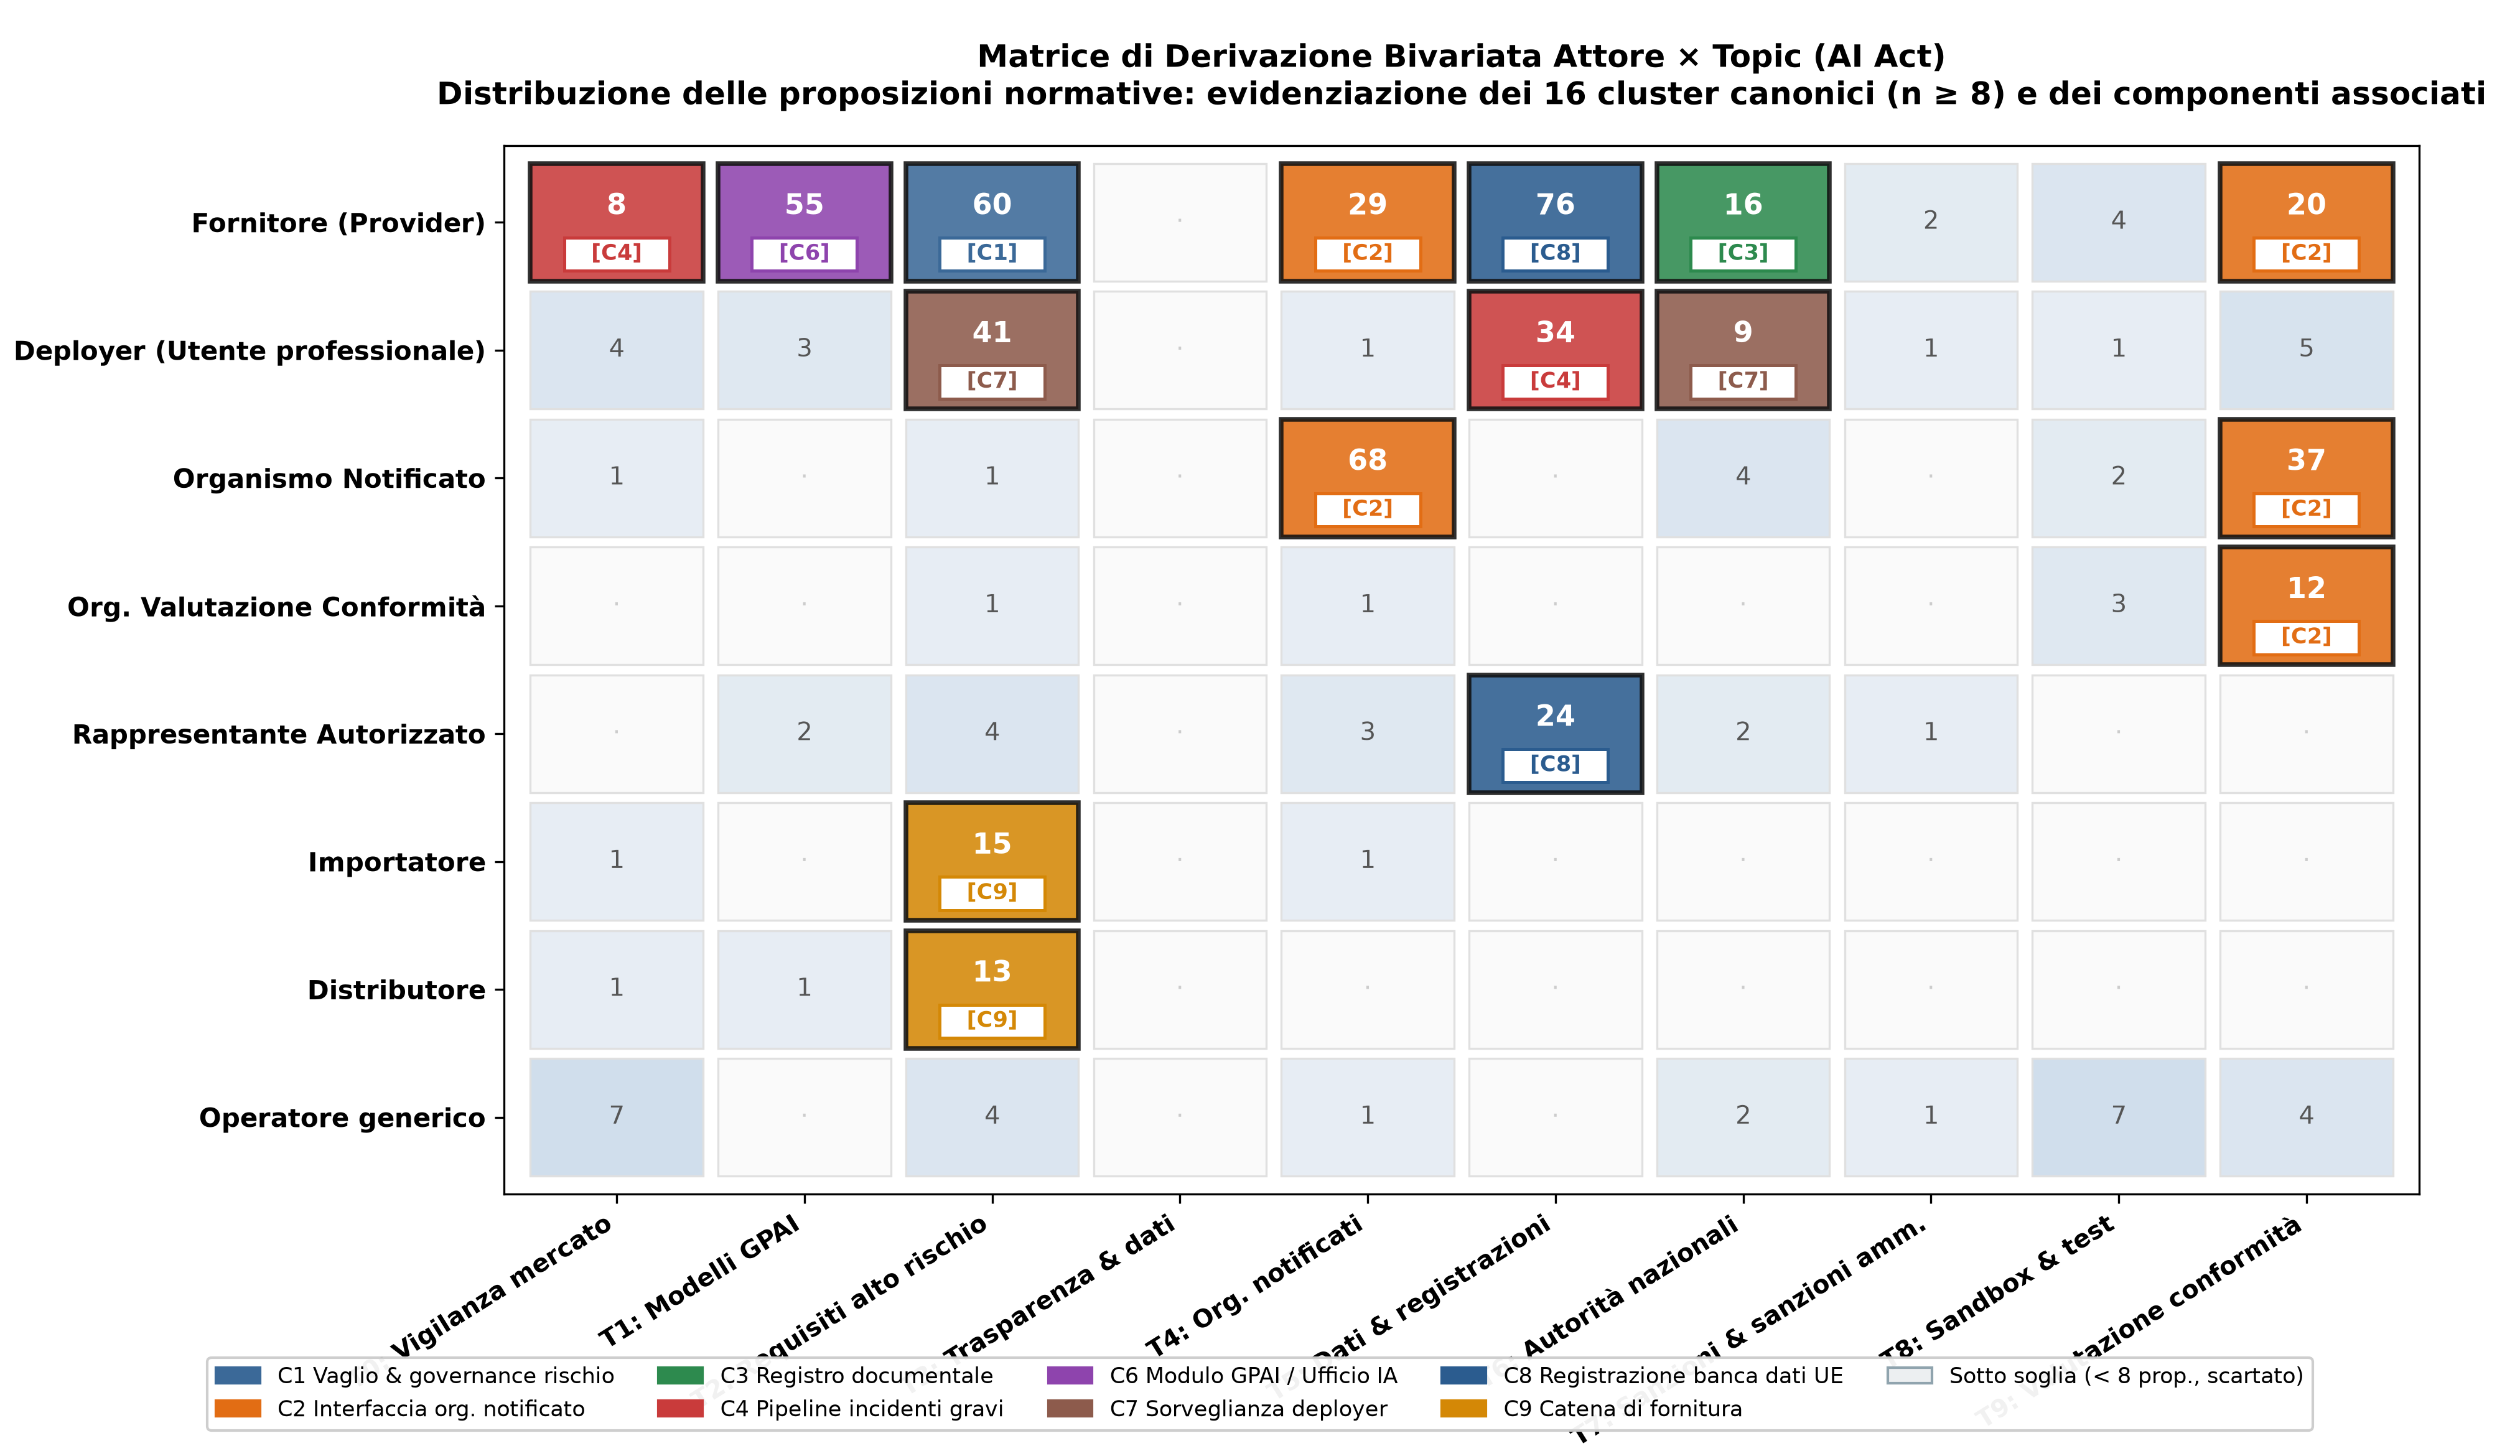
\includegraphics[width=\textwidth]{heatmap_attore_topic.png}
    \caption{Matrice di co-occorrenza $8 \times 10$ ($n \ge 8$).}
    \label{fig:heatmap_attore_topic}
  \end{subfigure}
  \hfill
  \begin{subfigure}[b]{0.49\textwidth}
    \centering
    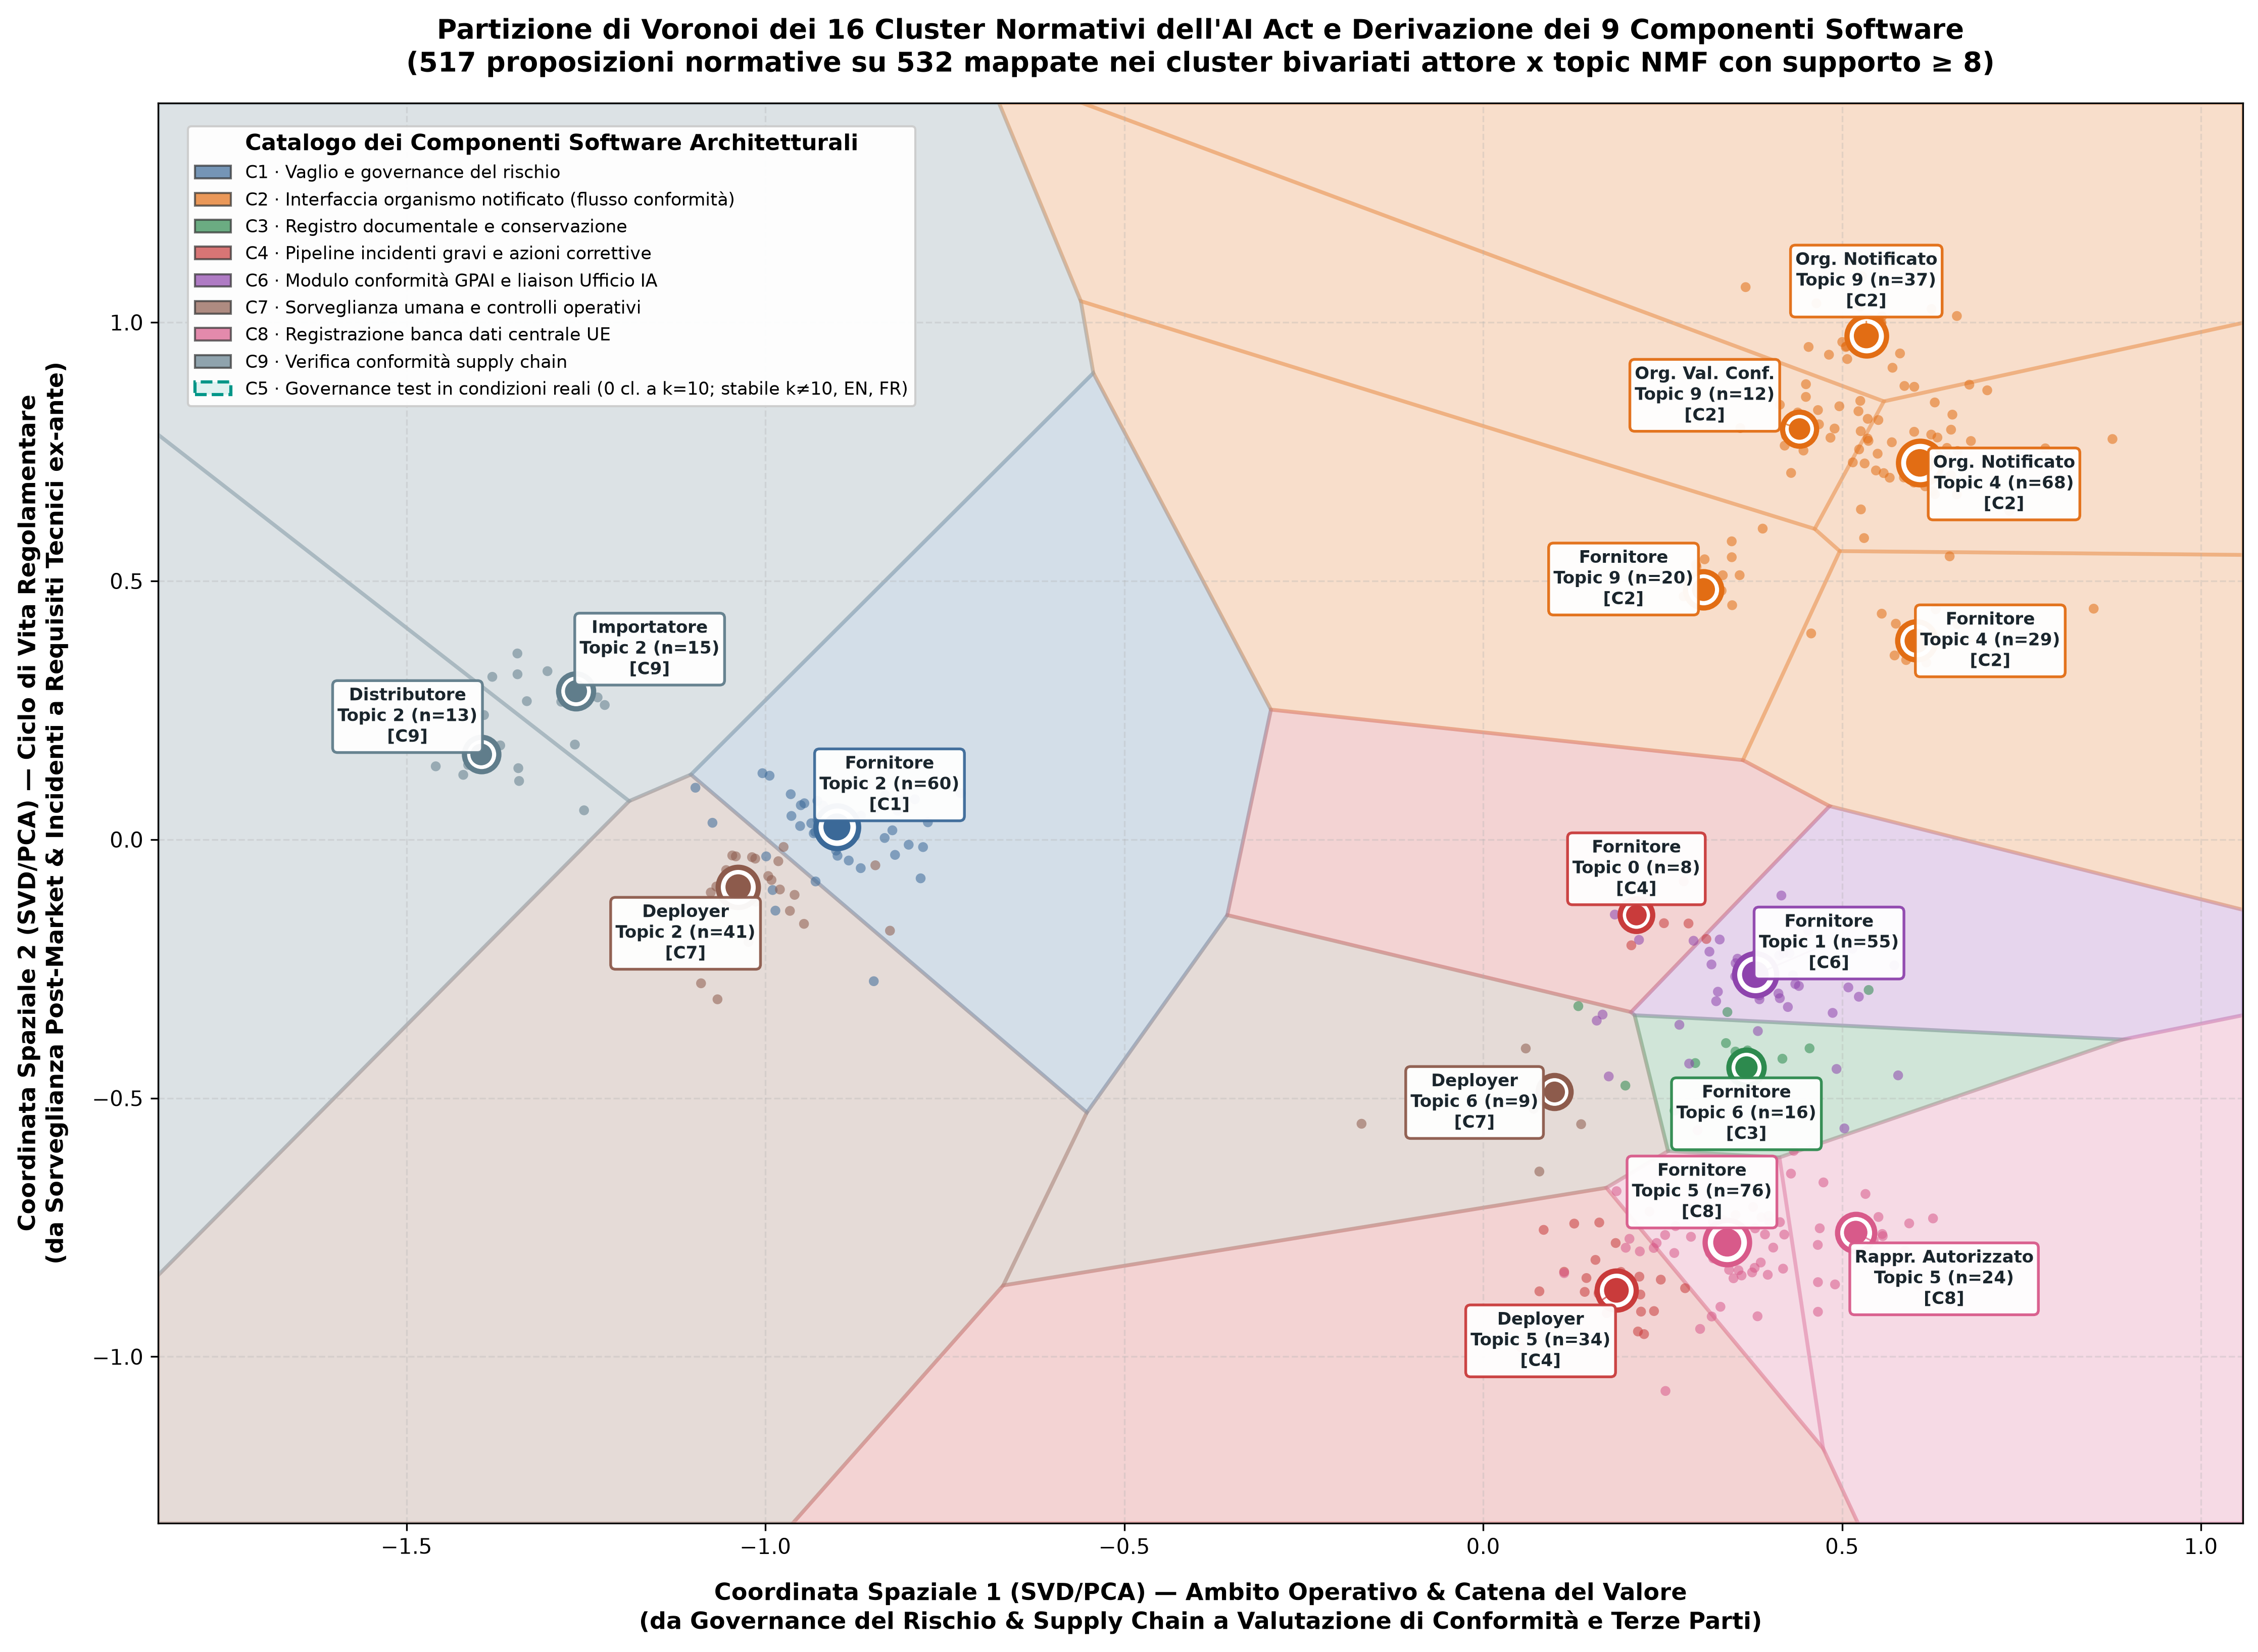
\includegraphics[width=\textwidth]{cluster_voronoi}
    \caption{Tassellazione di Voronoi dei 16 cluster.}
    \label{fig:cluster_voronoi}
  \end{subfigure}
  \caption[Derivazione bivariata e tassellazione geometrica di Voronoi]{Derivazione dei cluster bivariati dell'AI Act: (a) matrice empirica Attore $\times$ Topic con evidenza dei 16 cluster sopra-soglia; (b) partizione geometrica di Voronoi nello spazio continuo dei requisiti, con aggregazione funzionale nei componenti software.}
  \label{fig:cluster_derivazione}
\end{figure}

A completamento della partizione poligonale, la \cref{fig:semantic_projection_2d} presenta la \textbf{proiezione semantica continua 2D delle \num{1171} proposizioni} (PCA sui vettori Topic $\times$ Attore): le ellissi di confidenza  ($1{,}4\,\sigma$) e i centroidi evidenziano la netta polarizzazione funzionale dei componenti del catalogo rispetto alle norme trasversali di contesto (in grigio).

\begin{figure}[htbp]
  \centering
  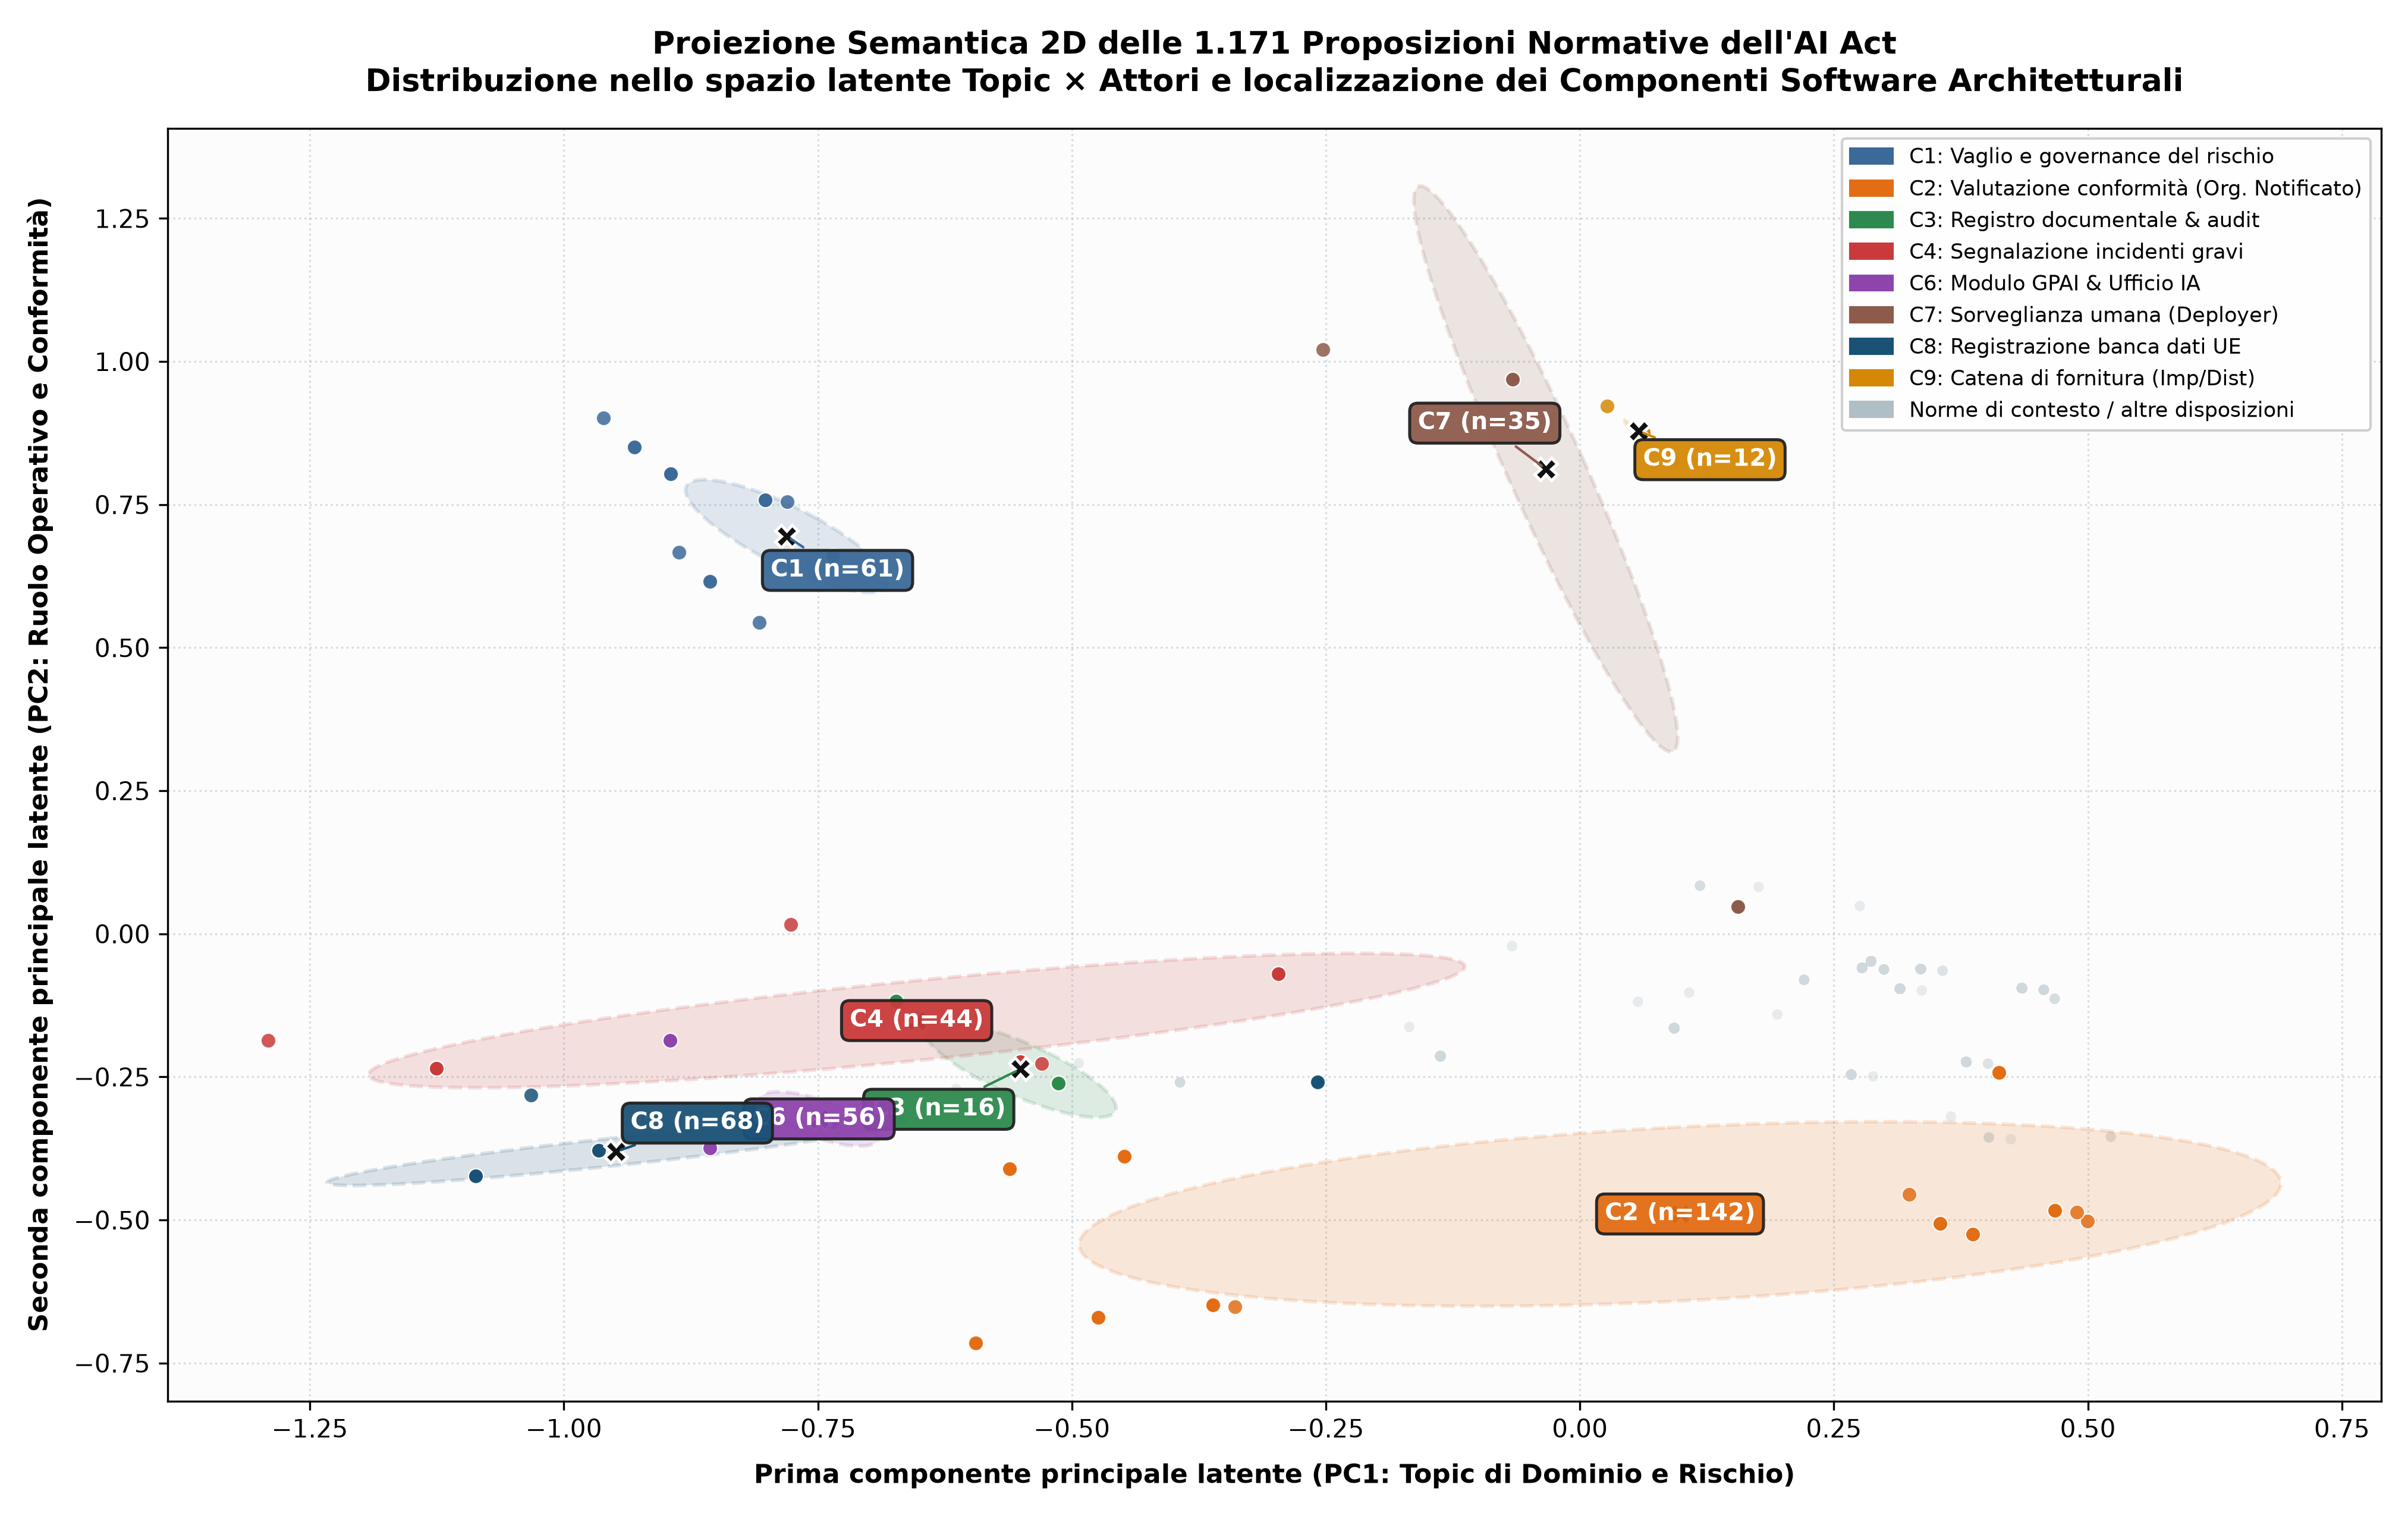
\includegraphics[width=0.76\textwidth]{semantic_projection_2d.png}
  \caption[Proiezione semantica continua 2D del corpus normativo]{Proiezione semantica continua 2D delle \num{1171} proposizioni dell'AI Act (PCA Topic $\times$ Attore). Le ellissi di confidenza mostrano l'autonomia funzionale dei cluster rispetto al substrato comune.}
  \label{fig:semantic_projection_2d}
\end{figure}

I 16 cluster bivariati si ricompongono nel \textbf{catalogo canonico dei 9 componenti software}(\cref{tab:catalogo_componenti}), coprendo l'intero ciclo di ivta del sistema di IA: 8 componenti sono direttamente sostenuti dai cluster in lingua italiana a $k = 10$ nelle versioni EN/FR ed in italiano variando $k$.

\begin{table}[htbp]
  \centering
  \small
  \caption[Il catalogo canonico dei 9 componenti software]{Il catalogo canonico dei 9 componenti software per la conformità all'AI Act (dettaglio dei singoli cluster in Appendice~\ref{app:catalogo}).}
  \label{tab:catalogo_componenti}
  \begin{tabularx}{\textwidth}{l X p{3.2cm} p{2.6cm} c r}
    \toprule
    \textbf{ID} & \textbf{Denominazione componente} & \textbf{Stadio ciclo vita} & \textbf{Attori responsabili} & \textbf{Clust.} & \textbf{Prop.} \\
    \midrule
    \textbf{C1} & Vaglio e governance del rischio & Sviluppo / classificazione & Fornitore & 1 & 60 \emph{(101)} \\
    \textbf{C2} & Interfaccia valutazione conformità & Valutazione conformità & Fornitore, CAB & 5 & 166 \\
    \textbf{C3} & Registro documentale e archivio & Valutazione conformità & Fornitore & 1 & 16 \\
    \textbf{C4} & Pipeline segnalazione incidenti & Monitoraggio post-market & Fornitore, Deployer & 2 & 42 \\
    \textbf{C5} & Governance test condizioni reali & Sviluppo / classificazione & Fornitore, Deployer & 0* & ---* \\
    \textbf{C6} & Modulo conformità GPAI & Sviluppo / classificazione & Fornitore GPAI & 1 & 55 \\
    \textbf{C7} & Sorveglianza umana e controlli & Monitoraggio post-market & Deployer & 2 & 50 \\
    \textbf{C8} & Registrazione banca dati UE & Immissione sul mercato & Fornitore, Rappr. & 2 & 100 \\
    \textbf{C9} & Verifica conformità supply chain & Immissione sul mercato & Importatore, Distr. & 2 & 28 \\
    \bottomrule
  \end{tabularx}
\end{table}

\subsection{Quantificazione dell'eredità: Articolo 10 e Sezione 2 (Risposta a \texorpdfstring{$\mathcal{D}_2$}{D2})}
La quantificazione algebrica del principio di autosufficienza mediante l'operatore di chiusura di Galois sul reticolo formale risponde direttamente alla domanda $\mathcal{D}_2$:
\begin{enumerate}
    \item \textbf{Articolo 10 (Governance dei dati e data management)}: il sotto-reticolo generato dalle 24 proposizioni dell'art.~10 isola 14 intent formali. Di queste, ben \textbf{16 proposizioni (il \SI{66,7}{\percent})} sono completamente autosufficienti per isolamento sintattico e pertinenza semantica, mentre 8 proposizioni ereditano attributi di contesto (in particolare \campo{has_autorita} e requisiti generali di auditabilità) dal sovra-concetto di sezione.
  \item \textbf{Analisi di Sezione 2 (Requisiti per sistemi ad alto rischio, Artt.~8--15)}: come evidenziato empiricamente dalla \cref{fig:precipizio_sezione2}, la densità di rinvii interni e di dipendenze esterne mostra un tipico andamento a \enquote{precipizio}: l'Articolo 9 (sistema di gestione dei rischi, 18 collegamenti espliciti) e l'Articolo 10 (governance dei dati, 14 collegamenti) concentrano il \SI{61,5}{\percent} delle dipendenze funzionali dell'intero Capo III, fungendo da snodo architetturale obbligato per tutti i successivi obblighi di trasparenza, accuratezza e robustezza cibernetica.
\end{enumerate}

\begin{figure}[htbp]
  \centering
  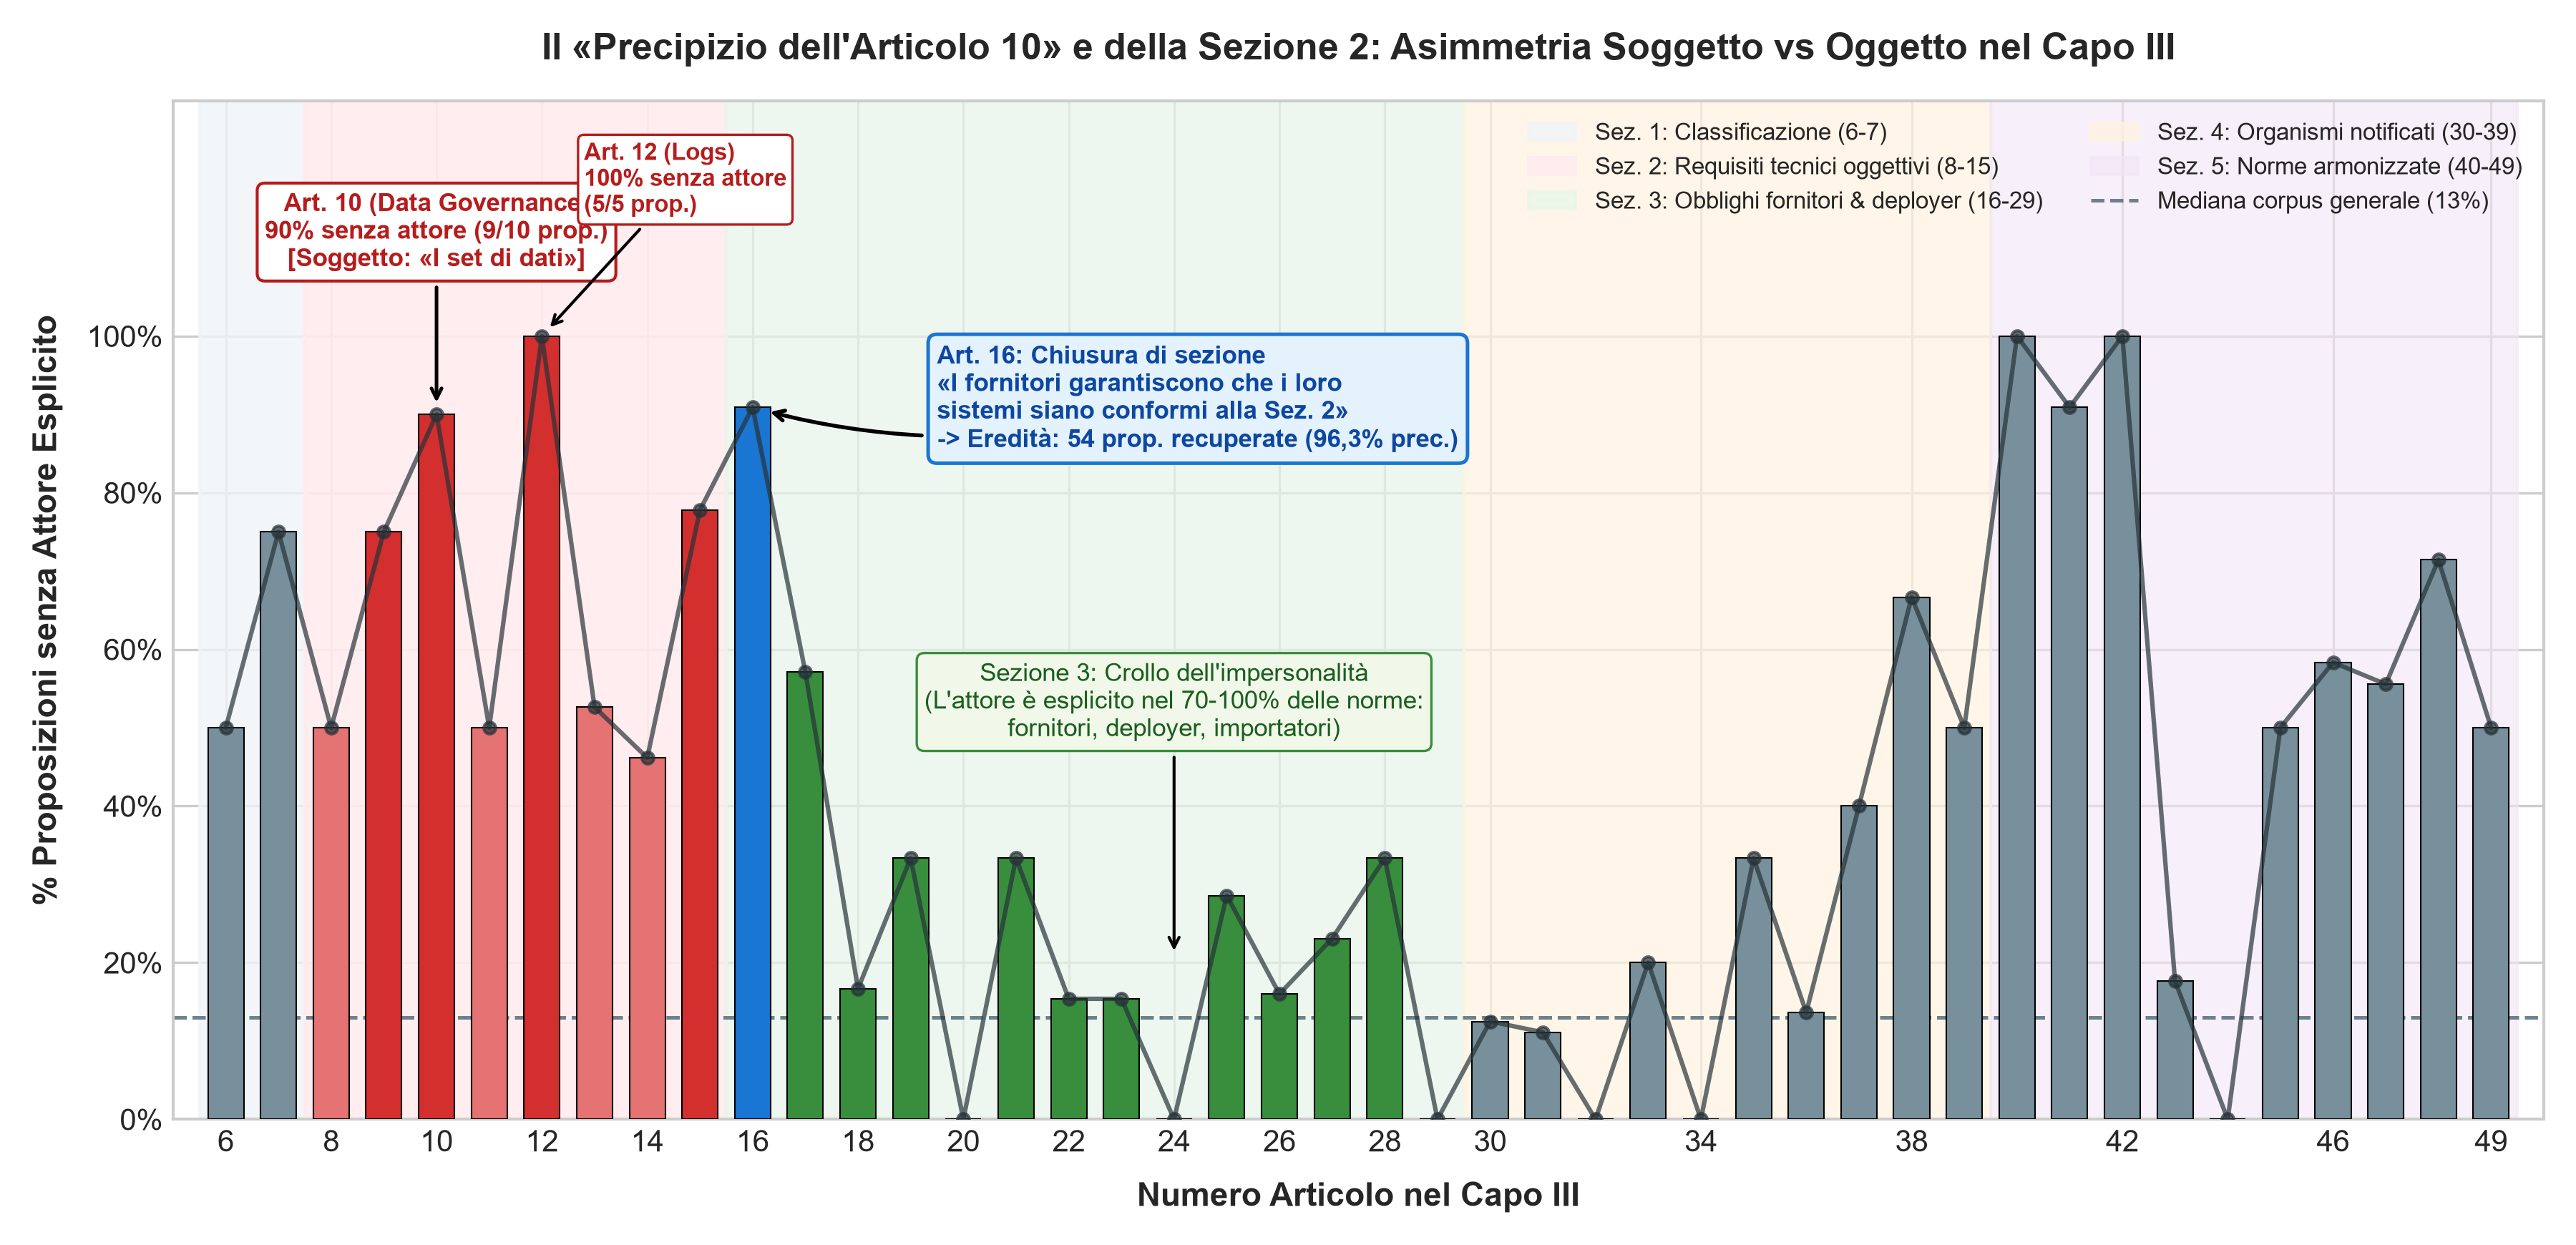
\includegraphics[width=0.76\textwidth]{precipizio_sezione2}
  \caption[Distribuzione delle dipendenze funzionali nella Sezione 2]{Distribuzione delle dipendenze funzionali nella Sezione 2 (Artt.~8--15): evidenza empirica della concentrazione degli obblighi sugli Artt.~9 e 10.}
  \label{fig:precipizio_sezione2}
\end{figure}

\subsection{{Robustezza multilingue e stabilità parametrica (Risposta a \texorpdfstring{$\mathcal{D}_3$}{D3})}}
\begin{enumerate}
    \item \textbf{Invarianza al modello NER}: rigenerando la matrice FCA e i cluster bivariati sostituendo le regole con le predizioni del modello Legal-BERT, tutti i 16 componenti sopra la soglia ed i 9 componenti risultano identici con identico supporto.
    \item \textbf{Stabilità Bootstrap}: sottoponendo il corpus a 30 ricampionamenti casuali al 90\%, i 16 cluster compaiono stabilmente in 28 run su 30, con indice di Jaccard medio $> 0,82$.
    \item \textbf{Analisi comparativa multilingue e sensibilità su $k$}:
    \begin{itemize}
        \item Nelle versioni in lingua inglese (\num{1330} proposizioni) e francese (\num{1223} proposizioni), emergono 18 cluster sopra-soglia che coprono i 9 componenti (incluso C5 già a $k=10$);
        \item Variando $k \in [7, 14]$ su tutte le lingue, il componente C5 si isola come cluster autonomo in 21 configurazioni sulle 24 totali (emerge stabilmente per $k \in [8, 14]$ in italiano e per ogni $k \ge 7$ in EN e FR), provando così che C5 rappresenta una reale funzione architetturale e non un artefatto dovuto alla segmentazione.
    \end{itemize}
\end{enumerate}

\end{document}